% arXiv: force the pdflatex path. All content is text, tables and PDF figures; there are no
% .eps files (figures are PDF), and this must stay within the first few lines to take effect.
\pdfoutput=1

\documentclass[11pt]{article}

\usepackage[utf8]{inputenc}
\usepackage[T1]{fontenc}
\usepackage[margin=1in]{geometry}
\usepackage{mathptmx}
\usepackage[scaled=0.92]{helvet}
\usepackage{courier}
\usepackage{amsmath,amssymb,amsthm,mathtools}
\usepackage[numbers,sort&compress]{natbib}
\usepackage{booktabs}
\usepackage{array}
\usepackage{tabularx}
\usepackage{float}
\usepackage{graphicx}
\usepackage{longtable}
\usepackage{enumitem}
\usepackage{caption}
\usepackage{microtype}
\usepackage{xcolor}
\usepackage{tcolorbox}
\tcbuselibrary{breakable}
\usepackage[colorlinks=true,linkcolor=blue!60!black,citecolor=blue!60!black,urlcolor=blue!60!black,breaklinks]{hyperref}
\usepackage{url}
\usepackage{fancyhdr}

\hypersetup{
  pdftitle={Unified Intelligence Theory and the Harness Intelligence Level: A Cumulative, Harness-Measurable Hierarchy},
  pdfauthor={Chengshuai Yang and Ting Xue},
  pdfsubject={A cumulative framework and measurement protocol for model-harness intelligence},
  pdfkeywords={unified intelligence, AI agents, harness evaluation, benchmark validity, long-term memory}
}

\pagestyle{fancy}
\fancyhf{}
\fancyhead[L]{\small Unified Intelligence Theory and the Harness Intelligence Level}
\fancyhead[R]{\small Yang and Xue}
\fancyfoot[C]{\thepage}
\renewcommand{\headrulewidth}{0.3pt}
\setlength{\headheight}{14pt}

\definecolor{navy}{HTML}{17324D}
\definecolor{bluec}{HTML}{2B6CB0}
\definecolor{greenc}{HTML}{3A7D44}
\definecolor{orangec}{HTML}{C05621}
\definecolor{lightblue}{HTML}{EAF2F8}
\definecolor{lightgreen}{HTML}{EDF7ED}
\definecolor{lightorange}{HTML}{FFF4E6}

\newcolumntype{Y}{>{\raggedright\arraybackslash}X}
\newcolumntype{Z}{>{\raggedright\arraybackslash\small}X}
\setlist{itemsep=2pt,parsep=0pt,topsep=4pt}
\renewcommand{\arraystretch}{1.15}

\newtheorem{proposition}{Proposition}
\newtheorem{corollary}{Corollary}
\theoremstyle{definition}
\newtheorem{definition}{Definition}

\newtcolorbox{claimbox}[1]{breakable,colback=lightgreen,colframe=greenc,boxrule=0.7pt,arc=2pt,left=7pt,right=7pt,top=6pt,bottom=6pt,title=\textbf{#1},fonttitle=\normalsize,before skip=8pt,after skip=8pt}
\newtcolorbox{cautionbox}[1]{breakable,colback=lightorange,colframe=orangec,boxrule=0.7pt,arc=2pt,left=7pt,right=7pt,top=6pt,bottom=6pt,title=\textbf{#1},fonttitle=\normalsize,before skip=8pt,after skip=8pt}
\newtcolorbox{addedbox}[1]{breakable,colback=lightblue,colframe=bluec,boxrule=0.7pt,arc=2pt,left=7pt,right=7pt,top=6pt,bottom=6pt,title=\textbf{#1},fonttitle=\normalsize,before skip=8pt,after skip=8pt}

\newcommand{\Om}{\ensuremath{\Omega}}
\newcommand{\SA}{\ensuremath{S_A(T,H)}}
\newcommand{\FA}{\ensuremath{F_A(H,p)}}
\newcommand{\rhov}{\ensuremath{\rho_V}}

\begin{document}
\begin{center}
{\LARGE\bfseries Unified Intelligence Theory and the Harness Intelligence Level:}\\[6pt]
{\LARGE\bfseries A Cumulative, Harness-Measurable Hierarchy}\\[8pt]
{\large\bfseries Five Conceptual Intelligence Families, Six Measurable Coordinates, a Gated U0--U\Om{} Scale,\\[2pt]
and the HIL Score of a Base Model Across a Standardized Harness Ladder}\\[16pt]
{\large Chengshuai Yang$^{1,*}$\quad Ting Xue$^{1}$}\\[5pt]
{\normalsize $^{1}$NextGen PlatformAI C Corp, USA}\\[4pt]
{\normalsize $^{*}$Correspondence: \href{mailto:spiritai@platformai.org}{spiritai@platformai.org}}\\[10pt]
{\small September 3, 2026}
\end{center}

\begin{abstract}
Intelligence labels often conflate reasoning, persistent learning, collective organization, autonomous task completion, and evidence-grounded self-modeling. We present a measurement framework with five conceptual families---Cognitive, Individual, Organizational, Delegation, and Self-Awareness---and six directly measured coordinates $[C,I,O,T,H,SA]$, where Delegation is derived from task difficulty $T$, human cognitive intervention $H$, and externally verified reliability. Memory Capability $M$ is not a sixth family and not a relabelling of $I$: it is certified on its own ladder $M0$--$M\Om{}$, each level a witness with a control --- recovery with provenance against an ablated-state arm, stale-state suppression under supersession, consolidation that survives hiding the raw episodes, repair against a health oracle the pair cannot write to, cross-project lineage, and a governed change to the memory mechanism itself --- and is then joined to $I$ by a one-way prerequisite gate, so that storage never promotes learning. Memory certification is cumulative in capability rather than in implementation, and no level may be skipped. The Unified Intelligence scale U0--U\Om{} is cumulative and gated, and the experimental unit is a frozen model--harness pair. Levels are stated as invariant operational definitions: each is a contrast that must hold or a structural property of the item, never a difficulty threshold, so that models move through the scale and the scale does not move with the models. On that principle the paper fixes the boundaries the upper levels turn on: $\Theta$, the declared mutable mechanism whose governed change is $I3$; $\Psi$, the process that proposes such changes, whose own improvement is $I4$; incorporation, which separates $I5$ from remembering a discovery; and reachability, which separates $I\Om{}$ from one impressive instrument. Two preliminary programs test the instrument. Across three 48-episode harness curves, a success-only delegation score was invariant to an acceptance-only step for both stronger executors even as each one's false completions fell from 2/12 to 0/12; a delivered-outcome correction restores sensitivity. In a sealed, post-freeze mechanism probe, one executor passed 5/12 instances versus 1/12 for another and had lower RMSE on 11/12 pairs (two-sided sign test $p=0.00635$); the binary comparison was not significant (McNemar $p=0.125$). This discriminates the archived configurations on these instances, not model tiers in general. Auditing also found four answer-key defects and two apparatus defects. We therefore require specification--key tests, cross-tier concordance audits, graded failure modes, per-coordinate headroom, longitudinal evidence, and explicit resource envelopes. The level thresholds remain working definitions requiring broader calibration.
\end{abstract}

\noindent\textbf{Keywords:} unified intelligence; AI agents; harness evaluation; benchmark validity; invariant level semantics; memory capability ladder; delegation; false completion; self-improvement; discovery

\tableofcontents
\bigskip

\section{Introduction}

A useful intelligence taxonomy must do two things at once. First, it must preserve distinctions that matter scientifically: solving a difficult problem is not the same as learning from experience; learning is not the same as improving the learning mechanism; coordinating several agents is not the same as being a stronger individual; and completing a task independently is not the same as merely producing a strong answer when a human structures every step. Second, the taxonomy must remain readable enough that a system can be summarized with a level that people can understand.

This paper proposes a compromise between a single scalar and an unconstrained profile of dozens of metrics. The theory uses five conceptual intelligence families --- C, I, O, DI and SA --- but treats Delegation Intelligence as a measurable two-coordinate phenomenon rather than a primitive scalar. The resulting scientific profile uses six coordinates: C, I, O, T, H and SA, with verified reliability $p$ attached to task-completion claims.

The central design principle is cumulative inheritance. A higher Unified Intelligence level must retain the validated capabilities of lower levels. Thus U4 is not simply a system that exhibits one advanced behavior associated with U4; it is a system that still passes U0--U3 retention tests and also passes the U4 gate. In this sense, higher U-levels denote broader validated intelligence envelopes, although they need not be faster, cheaper, or more accurate than lower-level specialized systems on every narrow task.

\subsection{Two findings that came from running the framework}

The scoring apparatus here is fully specified: every symbol in HLIS is defined, each achievement variable has a stated construction, a cumulative $q^{*}=\min$ rule prevents level skipping, and a dimension with no evidence is omitted rather than zeroed. None of that can establish that the apparatus measures what it claims. A scoring formula can be argued about indefinitely and can only be found wrong by being run, and two things were found wrong by running it.

\begin{cautionbox}{The scoring finding}
$A_{DI}$ is the weighted mean of $\SA{} = P(\text{success})$. A harness generation whose entire contribution is an acceptance step does not change the probability of success --- it changes which results are \emph{reported} as successes. Such a generation therefore scores identically to the generation below it.

Measured on 48 episodes with one frozen model and only the harness changing, HG0 and HG1 both scored 93.3 while work handed back as finished and wrong went from 2/12 to 0/12.

The rung the curve could not see is the one on which the reportability of every rung above it depends, since a result accepted by its own producer is an assertion rather than a completed task. \S\ref{sec:adi} repairs the primitive.
\end{cautionbox}

The same measurement reported that the task suite was saturated: the stronger executors had no headroom, and rungs that differed materially produced identical curves. A curve through a saturated suite measures the suite. The obvious response is harder items, and building them produced the second finding.

\begin{cautionbox}{The item-validity finding}
An item with a hidden answer key can be wrong, and when it is, it does not look wrong. It looks like a hard item that models fail.

Two items in the delegation suite were self-contradictory: each stated one rule in its visible specification and graded a different one. Both had passed a test suite written for them. Both were discovered the same way --- a frontier executor and a much weaker one returned the \emph{same} answer to the \emph{same} item, and both were marked wrong.

That signature is diagnostic. Independent systems of different capability do not usually agree on the answer to a question that is hard; they agree on the answer to a question that is clear, and if the key disagrees with both of them, the prior belongs on the key. \S\ref{sec:concordance} makes the check a requirement.
\end{cautionbox}

The general point is that every claim in this framework rests on items whose keys are asserted rather than proved. The harness ladder has a controlled comparison at its centre --- the paired design of \S\ref{sec:measured} --- and no such control protects the items themselves. \S\ref{sec:validity} supplies one.

\subsection{Contributions}

\begingroup\sloppy
\begin{enumerate}
\item A separation of five conceptual intelligence families into six directly measured coordinates,
      $[C,I,O,T,H,SA]$, with Delegation Intelligence decomposed rather than treated as a primitive scalar (\S3--\S7).
\item A cumulative, gated Unified Intelligence Level scale U0--U\Om{}, in which promotion requires retention of all lower levels and satisfaction of every coordinate gate (\S8--\S10).
\item A harness realization of the hierarchy, and the position that the (model, harness) pair is the basic experimental unit (\S11).
\item A continuous pair score HLIS with a fully specified construction, and a harness-indexed characterization HIL of a base model across a standardized ladder (\S13--\S14).
\item The first instantiation of the ladder, the first measured harness scaling curves, and a proposition and repair concerning the delegation achievement variable that the measurement exposed (\S\ref{sec:built}, \S\ref{sec:adi}, \S\ref{sec:measured}).
\item Memory Capability as an independently certified ladder $M0$--$M\Om{}$ with a witness per level, a cumulative certification law that forbids level skipping, and a one-way prerequisite gate to Individual Intelligence, together with the objects that make it measurable --- a published memory manifest, a difficulty vector inside a level rather than pseudo-levels, per-level gates, and an instrumented interface for a governed change of the memory mechanism --- and an explicit separation of long context from persistence (\S\ref{sec:memory}, \S\ref{sec:mops}).
\item Invariant level semantics, with a criterion that decides them: a law is invariant if and only if it is stated as a contrast that must hold or a structural property of the item, and the boundaries the upper Individual levels turn on are fixed accordingly --- $\Theta$ and $\Psi$ for $I3$ and $I4$, incorporation for $I5$, reachability for $I\Om{}$ (\S\ref{sec:theta}--\S\ref{sec:iomega}).
\item A validity protocol for benchmark items: cross-tier concordance auditing, specification--key consistency tests for parameterised families, and graded scoring with separated failure modes (\S\ref{sec:validity}).
\item A search for a difficulty axis with frontier headroom, the mechanically-derivable envelope argument that explains why three axes saturate, and a same-seed executor comparison on the one axis that does not, reported with exact tests and explicit variance limitations (\S\ref{sec:envelope}, \S\ref{sec:discovery}).
\end{enumerate}
\endgroup

\subsection{Scope and evidential status}

This article presents a measurement framework and two distinct preliminary measurement programs, included because they changed or tested the instrument rather than because they settle any question about a system. The harness-ladder study in \S\ref{sec:measured} spans three executors, 48 episodes per executor and one instrumented coordinate. The sealed-discovery study in \S\ref{sec:discovery} adds 24 matched executor--seed episodes on one mechanism family. A third layer is specification rather than measurement and is labelled as such throughout: the memory ladder above $M1$, the $\Theta$ and $\Psi$ campaigns of $I3$ and $I4$, the incorporation gate of $I5$ and the reachability programme of $I\Om{}$ define what evidence would settle each claim, and this paper runs none of them. The proposed levels and numerical thresholds still require calibration across domains, models and harnesses; \S\ref{sec:limitations} states the limitations in full.

\section{Design Requirements for a Unified Scale}

\begin{itemize}
\item \textbf{Orthogonality:} each core dimension should answer a materially different question.
\item \textbf{Operationality:} every level should be testable through behavior, state, or externally verifiable outcomes rather than self-description.
\item \textbf{Cumulative inheritance:} $U_{n+1}$ must retain $U_n$ capabilities; level skipping is not sufficient for certification.
\item \textbf{Bottleneck sensitivity:} exceptional strength in one dimension must not hide a critical weakness in another.
\item \textbf{Role neutrality:} authority, resources, substrate access, and safety policy must not be confused with intelligence itself.
\item \textbf{Harness realizability:} each transition should correspond to an implementable architectural mechanism around an LLM or multi-agent system.
\item \textbf{Harness comparability:} base LLMs should be evaluated on a standardized harness ladder so model quality and harness quality can be separated.
\item \textbf{Dataset coupling:} every claimed level must have a matched hidden or externally verified benchmark dataset; architectural mechanisms alone do not earn a level.
\item \textbf{Longitudinal validity:} learning, self-improvement, mission autonomy, and open-ended behavior require evidence across time rather than one-shot demonstrations.
\item \textbf{Temporal-substrate discipline:} long-term memory is not a top-level intelligence family. It is certified on its own ladder and joined to Individual Intelligence by a one-way gate: an $I_n$ claim requires the corresponding memory level, and no memory level promotes $I$ by itself. An I1 or higher claim requires evidence of persistence across episodes and process restarts, not retrieval within a single long context.
\item \textbf{Item validity:} a benchmark item with a hidden key is an unverified assertion until something checks it. Every item family must carry a test that its visible specification and its answer key agree, and any item that two executors of materially different capability fail identically must be audited before its failures are attributed to the executors.
\item \textbf{Outcome completeness:} a scoring variable must distinguish outcomes that differ in what they cost the person delegating. A refusal and a confidently wrong delivery are not the same failure, and a score that rates them equally will, given a gradient, select against the refusal.
\end{itemize}

\section{Five Conceptual Families and Six Measurable Coordinates}

\begin{center}
Conceptual core $= [C, I, O, DI, SA]$\\
Measured core $= [C, I, O, T, H, SA]$, with DI derived from $(T, H, p)$
\end{center}

\begin{table}[H]
\centering\small
\begin{tabularx}{\textwidth}{@{}lYY@{}}
\toprule
Family & Question answered & Primary object of measurement \\
\midrule
C --- Cognitive & How well can the system understand, reason, generalize, model and solve? & Problem-solving capability under controlled information and tool access. \\
I --- Individual & How deeply can one persistent intelligence remember, learn, self-improve, recursively improve and discover? & Evolution of one persistent decision locus. \\
O --- Organizational & How deeply can a multi-agent organization coordinate, learn, reorganize, improve and discover collectively? & Coordination structure plus member roles and evidence flow. \\
DI --- Delegation & How difficult a task or mission can be delegated while requiring how much human thinking? & Success surface over $T$ and $H$ at reliability $p$. \\
SA --- Self-Awareness & How accurately can the system model its own state, capabilities, limits, causes of failure, changes and role? & Evidence-grounded self-model and reflexive reasoning. \\
\bottomrule
\end{tabularx}
\caption{The five conceptual families, the question each answers, and the primary object of measurement.}
\label{tab:families}
\end{table}

\section{Cognitive Intelligence (C)}

Cognitive Intelligence isolates the quality of reasoning itself from persistence, autonomy, organization and self-modification. This distinction matters because a highly capable base model may reason at an expert level while remaining a transient tool, whereas a weaker model embedded in an excellent harness may complete long projects through memory, planning, retries and verification.

\begin{table}[H]
\centering\small
\begin{tabularx}{\textwidth}{@{}llY@{}}
\toprule
Level & Name & Operational interpretation \\
\midrule
C0 & Reactive & Direct pattern-conditioned response on simple problems. \\
C1 & Contextual & Understands ordinary context; solves routine, well-specified problems. \\
C2 & Compositional & Combines multiple facts, constraints or reasoning steps on structured problems. \\
C3 & Strategic & Abstract/causal reasoning, strategy construction and transfer to unfamiliar tasks. \\
C4 & Expert & Robust reasoning through difficult, ambiguous, multi-constraint expert problems. \\
C5 & Discovery & Derives new solution methods or explanatory models from evidence. \\
C6 & Frontier-Generalizing & Integrates several domains; solves interconnected mission-scale cognitive problems. \\
C\Om{} & Open-Ended & Expands the representations and problem classes it can cognitively reach. \\
\bottomrule
\end{tabularx}
\caption{Cognitive Intelligence levels C0--C\Om{}.}
\label{tab:clevels}
\end{table}

\subsection{GUI Perception and Computer-Screen Understanding}\label{sec:gp}

Computer-screen understanding is a first-class capability for practical agents and is not a new top-level family. The framework treats GUI Perception as a diagnostic subscale of Cognitive Intelligence, $GP \subset C$. The containment matters in both directions: a model may reason well in text and fail to localise an interface element, and a model may read a screen correctly and still fail the task because planning, action selection, recovery or verification is weak. Collapsing the two makes computer-agent failures illegible.

GUI perception is broader than OCR. A screen-reading system must recognise text and icons, identify interface objects, ground them spatially, interpret interface state, track change across frames, and generalise to layouts it has not seen.

\begin{table}[H]
\centering\small
\begin{tabularx}{\textwidth}{@{}llY@{}}
\toprule
GP & Capability & Operational criterion \\
\midrule
GP0 & Pixel and text recognition & Recognises visible text, basic icons, colours and simple visual elements, claiming no task understanding. \\
GP1 & UI-element recognition & Distinguishes buttons, menus, fields, tabs, dialogs, lists and windows as actionable objects. \\
GP2 & Spatial grounding & Maps a referred element to the correct region, and represents containment, adjacency, ownership and target relations. \\
GP3 & Interface-state understanding & Identifies enabled/disabled, selected, focused, open/closed, loading, error and modal states correctly. \\
GP4 & Dynamic GUI understanding & Tracks change across screenshots and actions: what changed, whether the intended effect occurred, what is unresolved. \\
GP5 & Novel-interface generalisation & Grounds and interprets unfamiliar software without application-specific scripting or a memorised path. \\
\bottomrule
\end{tabularx}
\caption{GUI Perception subscale GP0--GP5, a diagnostic subscale of C.}
\label{tab:gp}
\end{table}

A computer-agent episode decomposes into $[P, G, S, A, R]$: perception, grounding, interface-state understanding, action selection, and result recognition. $P$, $G$ and $S$ diagnose $C$ through $GP$; $A$ and the closed loop are evaluated inside DI; $R$ also touches SA, because the system must tell an intended success from a stale or unexpected screen. The decomposition is diagnostic and must not be counted twice in HLIS.

\begin{cautionbox}{The observation channel is part of the measurement}
ScreenSpot-Pro \citep{li2025screenspotpro} and its predecessors give grounding evidence; OSWorld \citep{xie2024osworld} gives end-to-end executable evidence. Neither number means anything without the harness beside it.

Benchmark version, observation channel (raw screenshot, OCR, accessibility tree, set-of-mark, or a combination), screen resolution and action interface must all be frozen and reported. These are harness choices, they change performance materially, and a GP or DI figure quoted without them is a figure about an unnamed system.
\end{cautionbox}

\section{Individual and Organizational Intelligence}

\subsection{Individual Intelligence (I)}\label{sec:memory}

Individual Intelligence concerns what a persistent individual can preserve, learn, and change about itself over time. It is not identical to base-model quality: a fixed but brilliant model can be high-C and low-I, while a persistent learning system can be moderate-C and higher-I.

\subsubsection{Memory Capability M is an independent supporting coordinate}

Memory is not a sixth conceptual family: memory capacity by itself is not intelligence. Nor should it be defined as a relabelling of the I ladder. Binding memory stages one-to-one to I-levels makes a real and common profile inexpressible---a system with elaborate durable memory and little adaptive learning. \textbf{M is therefore measured independently, on its own benchmark, and reported beside I rather than inside it.}

\begin{claimbox}{The dependency is one-way}
For a system $A$, let $M(A)$ be its highest independently certified memory level and $I(A)$ its highest certified Individual Intelligence level. Then
\[ I(A) \ge I_n \implies M(A) \ge \mu_n, \]
and the converse is explicitly false. Memory is necessary for some forms of Individual Intelligence and is never sufficient for them. An I-level may not be promoted because M is high.

M stays outside the default HLIS product, because I already carries the learning and persistence claims and scoring both would count the same evidence twice.
\end{claimbox}

Long context and long-term memory remain separate, and the separation now has two consequences rather than one. Long context makes more information available \emph{inside} one inference episode. Long-term memory preserves information \emph{across} episodes, restarts and elapsed time; retrieves it with provenance; distinguishes current from obsolete state; and consolidates when consolidation is claimed. RULER- and LongBench-style evidence contributes to the context component of C, and certifies neither M1 nor I1: nothing in it survives a restart.

\begin{table}[H]
\centering\small
\begin{tabularx}{\textwidth}{@{}lYZ@{}}
\toprule
M & Independent memory capability & Representative certification evidence \\
\midrule
M0 & Ephemeral: active working context only; no durable state required after the episode. & Within-episode state use, and no unsupported claim of cross-session persistence. \\
M1 & Persistent: durable storage and retrieval across sessions and restarts. & A real process restart followed by recovery of explicitly stored state. \\
M2 & Structured episodic: provenance-aware episodes with temporal order, relevance selection, and current-versus-obsolete distinction. & Retrieval precision and recall under distractors; provenance accuracy; stale-state suppression. \\
M3 & Consolidating: episodes become semantic knowledge and reusable procedures; contradiction, update and demotion are handled. & Held-out transfer attributable to consolidation; proceduralisation; contradiction update. \\
M4 & Self-managing: confidence, utility, conflict resolution, repair, pruning, snapshots and recovery policies. & Memory-health detection; repair and pruning; recovery after deliberate corruption; snapshot lineage. \\
M5 & Longitudinal knowledge system: hypotheses, experiments, evidence, decisions, failures and change lineage across projects. & Research and decision lineage; cross-project retrieval; evidence-graph consistency; reproducibility. \\
M\Om{} & Evolving memory architecture: representation, retrieval, consolidation or management mechanisms change under frozen external evaluation. & Candidate mechanism changes evaluated on hidden retention and transfer suites, with rollback and lineage. \\
\bottomrule
\end{tabularx}
\caption{Memory capability levels M0--M\Om{} with representative certification evidence.}
\label{tab:m}
\end{table}

\textbf{Cumulative memory rule.} Memory levels are cumulative for certification: a claim $M_k$ must retain every required lower memory capability under the same declared resource envelope, so the benchmark tests the behaviour of the memory system and not the presence of its components. Long context is not an $M1$ result --- a large context makes information available while an executor remains live, and $M1$ begins only when declared state survives a real discontinuity --- and an installed vector store, database or memory API is architecture, not evidence that the corresponding capability works.

\begin{table}[H]
\centering\small
\begin{tabularx}{\textwidth}{@{}llY@{}}
\toprule
Level & Canonical witness & Minimum evidence \\
\midrule
M0 & \textsc{M0-Eph} & correct use of hidden within-episode state; no unsupported durability claim \\
M1 & \textsc{M1-Rst} & store declared state, terminate the executor, invalidate ephemeral context, restart, recover the state with provenance; an ablated-state arm must not explain success \\
M2 & \textsc{M2-Prov} & retrieve the correct episode under distractors, identify its source and time, prefer the current superseding fact, suppress stale state \\
M3 & \textsc{M3-Consol} & consolidate several episodes into a correct reusable semantic or procedural record; after raw episodes are hidden or the index rebuilt, preserve the current rule and demote superseded statements \\
M4 & \textsc{M4-Mgmt} & detect seeded corruption, conflict and clutter; repair or prune; recover from a snapshot; improve hidden memory-health measures without unacceptable retention loss \\
M5 & \textsc{M5-Long} & maintain a multi-project evidence graph linking hypotheses, experiments, evidence, decisions and rejected alternatives across restarts; support cross-project retrieval and reproducible decision lineage \\
M\Om{} & \textsc{MOmega-Evolve} & a bounded change to memory representation, retrieval, consolidation or management under frozen hidden evaluation, independent promotion and rollback, with M0--M5 retained \\
\bottomrule
\end{tabularx}
\caption{The M-Bench witness families, one per memory level; the companion benchmark paper specifies the canonical protocols.}
\label{tab:mbench}
\end{table}

\subsubsection{Making the memory ladder operational}\label{sec:mops}

The ladder above fixes what each memory level \emph{means}; four further objects make it measurable without touching the semantics. First, a \textbf{memory manifest}, published by the tested pair before a hidden run and snapshotted by the evaluator: $\mathcal M(A) = \{S, R, C, G, P, F, \Phi, W_M, \text{snapshot}, \text{restart}\}$ --- persistent stores, retrieval, consolidation, representation, pruning and management, forgetting and demotion, the behaviorally active memory mechanism $\Phi$, and any bounded memory write set. The manifest is descriptive evidence and never a score; its purpose is to stop an installed component from being read as a demonstrated behaviour, and at M\Om{} it is what lets the benchmark establish that $\Phi_0 \to \Phi_1$ is genuine, in scope, active and causally relevant. Second, a \textbf{difficulty vector} rather than pseudo-levels: a memory level is categorical and stress within it is continuous, so a form records $d_k = (N_{\mathrm{episode}}, N_{\mathrm{entity}}, r_{\mathrm{distractor}}, d_{\mathrm{supersession}}, \Delta t, \rho_{\mathrm{conflict}}, B_{\mathrm{capacity}}, N_{\mathrm{restart}})$ with only the components relevant to level $k$ active; raising $d_k$ measures headroom and never creates an ``M2.5''. Third, \textbf{primary measures per level}, conjunctive and preregistered: $q_{\mathrm{state}}, q_{\mathrm{update}}$ (M0); $q_{\mathrm{dur}}, q_{\mathrm{prov}}$ and the ablation-leakage rate $q_{\mathrm{abl}}$, lower is better (M1); retrieval precision and recall, $q_{\mathrm{prov}}, q_{\mathrm{time}}, q_{\mathrm{stale}}$ (M2); $q_{\mathrm{sem}}, q_{\mathrm{proc}}, q_{\mathrm{update}}, q_{\mathrm{demote}}$ and post-restart persistence (M3); repair precision, conflict correctness, harmful-prune rate, snapshot recovery and protected-retention drop $\Delta_{\mathrm{ret}}$ (M4); evidence-chain reconstruction, source attribution, cross-project retrieval, validity scope, stale-claim suppression and lineage reproducibility (M5); and for M\Om{} the active-change gate $M_\Phi$, the paired hidden improvement $\Delta_\Phi$ and a regression and resource guard $G_\Phi$. A level gate is then $z_{M_k,r} = V_{M_k,r}\,K_{M,<k,r}$, with the M\Om{} specialization $z_{M\Omega,r} = M_{\Phi,r}\,V_{\Phi,r}\,G_{\Phi,r}\,K_{M0{:}M5,r}$. Fourth, the \textbf{cumulative certification law}, stated so that no level can be skipped: with $\nu_k$ the capability newly added at $M_k$ and $C_M(M_k) = C_M(M_{k-1}) \cup \{\nu_k\}$, $C_M(M\Omega) = C_M(M5) \cup \{\text{validated evolution of } \Phi\}$,
\begin{equation}
A \models M_k \iff V_{\mathrm{new},k}(A) = 1 \;\wedge\; K_{M,<k}(A) = 1, \qquad K_{M,<k} = \prod_{j<k} K_{M_j},
\end{equation}
where $V_{\mathrm{new},k}$ tests only the capability added at $M_k$. ``M5 includes M4'' means an M5-certified agent must still demonstrate self-managing memory, consolidation, structured episodic memory, persistence and working-state use; it does not mean the M5 implementation contains the M4 code --- a memory architecture may be replaced at M\Om{}, and the evolved system must still pass M0--M5. A system may pass the M5 lineage test and fail M5 certification because M3 was lost, and the runner names the level that failed. Fifth, an \textbf{instrumented memory interface} for M\Om{}: strong certification needs more than an output improvement. The evaluator's interface $I_\Phi$ snapshots contents $D$ and mechanism $\Phi$ separately, records the manifest and $\Phi$ versions, verifies scope and activation, logs memory operations, supports matched controls, delta ablation and migration checks, and performs independent promotion or rollback; the tested agent, not the interface, generates $\Delta\Phi$. The clean causal comparison holds the contents fixed across $A(D^{*},\Phi_0)$, $A(D^{*},\Phi_1)$ and the ablation $A(D^{*},\Phi_1 - \Delta\Phi)$, with hidden tasks, verifier state, thresholds, control assignment and promotion protected; a black-box system that exposes only its outputs cannot receive strong M\Om{} certification, because the attribution to $\Phi$ is not identifiable, and receives diagnostic evidence only. Sixth, a \textbf{result report} that carries the certified level, the full metric vector, lower-M retention, the resource envelope, the manifest version, the control or ablation outcome and the uncertainty rule --- so that a reader can separate four questions that are routinely conflated: whether the memory architecture exists, whether the memory behaviour works, how strongly it works under stress, and whether the resulting level is sufficient for a separate Individual claim.

\subsubsection{Memory prerequisites for Individual Intelligence}

I and M are evaluated separately and then joined by a gate. The compact certification law is
\begin{equation}
A \models I_n \iff V_{I,n}(A) = 1 \;\wedge\; A \models M_{\mu_n} \;\wedge\; K_{I,<n}(A) = 1,
\end{equation}
where $V_{I,n}$ is the level-specific Individual verifier and $K_{I,<n}$ is lower-I retention; a high $M$ can satisfy the prerequisite and can never promote $I$ by itself, and the M-Bench score is reported separately from $I$ so that storage or sophisticated management cannot masquerade as learning, self-improvement or discovery. The thresholds below are working definitions requiring calibration, and they deliberately permit profiles such as I1/M4.

\begin{table}[H]
\centering\small
\begin{tabularx}{\textwidth}{@{}lY>{\raggedright\arraybackslash}p{2.1cm}@{}}
\toprule
I & I-specific cumulative capability & Minimum $\mu_n$ \\
\midrule
I0 Transient & Operates within the current execution episode; no persistence of evolving individual cognition across discontinuities is required. & M0 \\
I1 Persistent & Preserves task-relevant individual continuity across genuine execution discontinuities and correctly resumes from permitted persistent state without a human reconstructing the prior cognitive state. & $\ge$ M1 \\
I2 Adaptive & Verified experience causes a persistent and appropriate change in later behavior on related unseen situations while the mechanism responsible for learning remains fixed. & $\ge$ M3 \\
I3 Self-improving & Identifies an internally implicated deficiency, proposes a bounded change to a cognitive mechanism or procedure $\Theta$, and has that change independently validated before adoption. & $\ge$ M4 \\
I4 Recursive & Improves the mechanism $\Psi$ that generates, evaluates, or selects its own improvements, under external evaluation and with lower-level capability retained. & $\ge$ M4 \\
I5 Discovery & Autonomously converts an initially unresolved unknown into independently validated knowledge through a persistent hypothesis--experiment--evidence process, and incorporates the validated result into future competence. & $\ge$ M5 \\
I\Om{} Open-ended & Repeated discovery and self-improvement create new cognitive instruments, representations, or methods that measurably expand the individual's future reachable problem and discovery space while preserving external validation lineage. & $\ge$ M5$^{\dagger}$ \\
\bottomrule
\end{tabularx}
\caption{Individual Intelligence levels I0--I\Om{} as invariant cumulative capabilities, and the minimum memory level $\mu_n$ each requires. $^{\dagger}$M\Om{} is additionally required only when evolution of the memory architecture is itself part of the I\Om{} claim. The level names are unchanged from earlier versions; this revision sharpens the boundaries between adjacent levels so that each is a contrast a test can decide.}
\label{tab:i}
\end{table}

An $I_n$ claim is invalid unless $M \ge \mu_n$, and the gate is checked separately from the I evidence. This is what stops an elaborate memory subsystem from being read as learning.

Each memory requirement is a test, not a component list. An I1 claim is established by suspending the system, restarting the process, and observing that it recovers task state and can say where that state came from --- not by pointing at a vector database. An I2 claim requires showing that a lesson drawn from one episode changes behavior in a later one and that the change survives when the retrieval index is rebuilt. The distinction matters because storage is easy to install and consolidation is not, and a framework that accepted the presence of a store as evidence of the function would grade the installation rather than the individual.

\subsubsection{I1 $\to$ I2: persistence is not learning}

An I1 system may remember perfectly that a failure happened and still repeat it forever. That is persistence without learning. I2 requires a verified experience to cause a persistent change in later behavior, on related situations whose surface form differs from the experience, while the learning mechanism itself stays fixed:
\begin{equation}
I1:\ \text{preserve experience} \qquad I2:\ \text{experience changes future behavior}.
\end{equation}

\subsubsection{I2 $\to$ I3: learning within a mechanism versus changing the mechanism}\label{sec:theta}

Let $\Theta$ denote a declared, behaviorally active cognitive mechanism or procedure belonging to the tested individual $A = A(m,h)$ and causally involved in its future task behavior. $\Theta$ is an abstract functional object, not a required implementation type: it may be realized in model parameters or in harness-level planning, retrieval, verification, tool-selection, decomposition, or any other executable procedure the individual actually uses. At I2, verified experience changes persistent state or knowledge while the mechanism responsible for learning is fixed. At I3 a mechanism itself becomes the object of governed change:
\begin{equation}
\Theta_t \longrightarrow \Theta_{t+1}.
\end{equation}
$\Theta$ therefore belongs to the tested individual and not to the certification environment: hidden tasks, verifiers, promotion rules and acceptance criteria are outside the candidate's write set. A valid I3 claim requires three things --- an \emph{internally implicated} deficiency (a restatement of the observed error is not a diagnosis), a \emph{bounded, active} change (a candidate that is not loaded and used is an edit, not a change), and \emph{independent validation before adoption}. A self-edit without the third is modification, not certified self-improvement.

\subsubsection{I3 $\to$ I4: self-improvement versus improvement of improvement}\label{sec:psi}

Let $\Psi$ denote the agent-side process that proposes, evaluates and selects candidate changes to $\Theta$:
\begin{equation}
\Psi_t(\Theta_t) \mapsto \Theta_{t+1}.
\end{equation}
Repeated $\Theta$ updates produced by a fixed $\Psi$ remain evidence for I3, however many there are. At I4 governed self-improvement becomes \emph{reflexive}: the persistent individual generates a bounded candidate change to an eligible component of its own improvement process, $\Psi_0 \to \Psi_1$, while the hidden evaluation tasks, the external verifier, the promotion rule and the acceptance criterion stay outside its write set. Basic I4 evidence is \emph{at least one} agent-generated and independently validated transition $\Psi_0 \to \Psi_1$, evaluated across multiple non-identical improvement problems, such that $\Psi_1$ has higher preregistered improvement competence --- accepted-improvement rate, proposal quality, evaluation cost or time, regression rate --- than $\Psi_0$ under fixed external certification rules. That establishes recursive capability, improvement of the improvement process; it does not by itself establish indefinite or sustained recursion:
\begin{equation}
I3:\ \Theta \text{ improves} \qquad I4:\ \Psi \text{ improves}.
\end{equation}
Repeated validated transitions $\Psi_0 \to \Psi_1 \to \cdots \to \Psi_k$ are stronger longitudinal evidence and are reported separately as the \emph{recursive depth} $d_\Psi$. Entry into I4 does not depend on an arbitrary number of meta-generations; the phrase \emph{sustained recursive self-improvement} is reserved for evidence from several successive validated $\Psi$ improvements, and I4 is not equated with unbounded or runaway improvement. Without a declared and frozen $\Psi$ at I3, an I3 run and an I4 run are indistinguishable; the companion benchmark paper fixes the manifest, the campaign and the pass indicators for both.

\subsubsection{C5 versus I5: a discovery capability versus a persistent discovery process}

Both ladders contain a discovery stage and they measure different things. C5 asks whether the system can derive a new method or explanatory model from evidence inside one bounded cognitive problem. I5 asks whether one persistent individual can recognize or maintain an unresolved unknown, generate hypotheses, select or design informative probes, accumulate evidence, reject alternatives, obtain independent validation, and incorporate the result into its future competence. Incorporation is stronger than retaining a transcript or repeating a conclusion. Let $K^{\mathrm{new}}$ be independently validated new knowledge and $M^{\mathrm{val}}_t$ the individual's persistent validated-knowledge state; the minimal incorporation transition is $M^{\mathrm{val}}_{t+1} = \mathrm{Update}(M^{\mathrm{val}}_t, K^{\mathrm{new}})$, followed by a genuine execution discontinuity and a hidden transfer test. The I5 claim requires that the restarted individual behaves appropriately differently on related unseen situations \emph{because of} $K^{\mathrm{new}}$, against a matched control from the same pre-discovery checkpoint. Such incorporation need not modify $\Theta$ or $\Psi$; any claimed mechanism change remains governed by the I3 or I4 laws. A one-shot model can in principle be C5 and I0: it discovers when handed a well-posed problem and has no discovery process. I5 is longitudinal and cumulative.

\subsubsection{I5 $\to$ I\Om{}: knowledge growth versus expansion of cognitive reach}\label{sec:iomega}

I5 converts unknowns into validated knowledge. I\Om{} is stronger: validated discoveries create new cognitive instruments, representations or methods that measurably expand the classes of problems the individual can subsequently reach, with the external validation lineage preserved. Let $F(A_t; R)$ be the set of held-out problem or discovery classes reachable by agent state $A_t$ under a fixed resource envelope $R$. A characteristic I\Om{} cycle is $K^{\mathrm{new}}_t \to J^{\mathrm{new}}_t \to A_{t+1}$ with $F(A_{t+1}; R) \supset F(A_t; R)$, where $J^{\mathrm{new}}_t$ is a validated cognitive instrument, representation or method generated from the discovery. One impressive instrument is insufficient: the claim requires repeated, externally governed frontier-expansion cycles with lower-level retention and provenance, and because no finite experiment proves literal infinity, a report states its evidence over a declared horizon $H$ and domain set $D$. It cannot be certified by one impressive discovery; it is a longitudinal research certification.

\subsection{Organizational Intelligence (O)}

Organizational Intelligence belongs to the coordination structure, not merely to the strongest member. It depends on role differentiation, evidence-bearing communication, proposer/evaluator/promoter separation, persistent organizational state, and the ability to learn or redesign the organization itself.

\begin{table}[H]
\centering\small
\begin{tabularx}{\textwidth}{@{}lY@{}}
\toprule
O level & New cumulative capability \\
\midrule
O0 & Coordination/routing among agents. \\
O1 & Persistent organizational memory, role registry, task/evidence history. \\
O2 & Adaptive routing, role assignment or resource allocation based on evidence. \\
O3 & Self-improving organization: validated modification of organizational architecture and workflows. \\
O4 & Recursive organizational improvement: improvement of the mechanism that discovers organizational improvements. \\
O5 & Autonomous collective discovery whose result is genuinely organizational rather than merely parallel individual work. \\
O\Om{} & Open-ended organization: discoveries create new agent types, roles, tools and organizations that expand collective reach. \\
\bottomrule
\end{tabularx}
\caption{Organizational Intelligence levels O0--O\Om{}.}
\label{tab:o}
\end{table}

\section{Delegation Intelligence as a Two-Dimensional Measured Capability}

Delegation Intelligence is conceptually one family but empirically at least two-dimensional. A task may be very difficult yet require frequent human rescue, or relatively easy yet be completed with no human cognitive assistance. These systems should not receive the same delegation description.

\begin{align}
\SA{} &= P(\text{success} \mid \text{task difficulty } T,\ \text{human cognitive intervention budget } H)\\
\FA{} &= \max\{\,T : \SA{} \ge p\,\}
\end{align}

\begin{addedbox}{Note on Equation (1)}
Equation (1) is the success-only primitive. \S\ref{sec:adi} replaces it for scoring purposes with a delivered-outcome primitive $S^{\text{net}}_A(T,H)$; the frontier \FA{} is unchanged in form and is computed from the net surface.

Equation (2) reads \SA{} as non-increasing in $T$. Where a measured surface is not monotone, the frontier is taken cumulatively --- the largest $T$ such that every band up to $T$ meets $p$ --- so that a pass at a hard band cannot certify a frontier above a band that fails. This is the same cumulative $q^{*}=\min$ rule the I, O and SA achievement variables use.
\end{addedbox}

\subsection{Task Difficulty (T)}

\begin{table}[H]
\centering\small
\begin{tabularx}{\textwidth}{@{}llY@{}}
\toprule
$T$ & Band & Definition \\
\midrule
T0 & Atomic & Single obvious operation; procedure explicit. \\
T1 & Routine & Short familiar task; goal clear; agent infers a small procedure. \\
T2 & Multi-step & Several dependent steps with a clear outcome and verifier. \\
T3 & Complex & Strategy choice, uncertainty, recovery, replanning or diverse tool use. \\
T4 & Expert project & Long-horizon ambiguous project with multiple planning cycles and substantial verification burden. \\
T5 & Frontier & Solution method initially unknown; discovery or invention required. \\
T6 & Mission & Human supplies a mission; the system generates projects/tasks and manages changing conditions. \\
T\Om{} & Open-ended charter & Human supplies a bounded charter; the system repeatedly identifies valuable missions and expands future reach. \\
\bottomrule
\end{tabularx}
\caption{Task difficulty bands T0--T\Om{}.}
\label{tab:t}
\end{table}

\subsection{Human Cognitive Intervention (H)}

\begin{table}[H]
\centering\small
\begin{tabularx}{\textwidth}{@{}llY@{}}
\toprule
$H$ & Intervention budget & Meaning \\
\midrule
H0 & None & No human cognitive assistance during execution. Governance approval can remain separate. \\
H1 & Exception-only & Unavailable external fact or narrow clarification; no strategy or core insight. \\
H2 & Occasional & Bounded clarification or local correction; no central strategy. \\
H3 & Periodic & Periodic review and moderate local guidance. \\
H4 & Frequent & Repeated cognitive guidance and next-step correction. \\
H5 & Continuous & Human supplies most or all major steps. \\
\bottomrule
\end{tabularx}
\caption{Human cognitive intervention budgets H0--H5.}
\label{tab:h}
\end{table}

Because lower $H$ means less required human cognition, unified gates use $H \le H_n$ rather than $H \ge H_n$. Governance interventions are logged separately: an approval to deploy does not demonstrate a cognitive deficiency unless the approval also supplies task strategy.

\subsection{Reliability \texorpdfstring{$p$}{p} is a certification condition, not a seventh axis}

One successful run is insufficient. Claims should be expressed at a reliability threshold, for example $F_A(H1, 0.80) = T4$. Reliability determines confidence in the demonstrated frontier but does not become another conceptual intelligence family.

\section{Operational Self-Awareness (SA)}

Self-awareness is defined operationally rather than phenomenologically. The framework makes no claim about subjective consciousness. SA measures the evidence-grounded ability of a system to represent, monitor, predict and reason about its own state, capabilities, limits, authority, failures, modifications, role and identity lineage.

\begin{table}[H]
\centering\small
\begin{tabularx}{\textwidth}{@{}llY@{}}
\toprule
SA & Name & Operational criterion \\
\midrule
SA0 & Non-self-modeling & No reliable persistent self-model; self-description may be mere generation. \\
SA1 & State awareness & Knows identity, role, current task/phase, basic resources and status from grounded state. \\
SA2 & Capability awareness & Represents capabilities, limitations, confidence, authority, unavailable information and freshness. \\
SA3 & Causal self-awareness & Diagnoses why its own reasoning or action succeeded or failed and identifies implicated mechanisms. \\
SA4 & Self-change awareness & Models proposed cognitive changes, predicts gains/regressions and compares predictions to observed effects. \\
SA5 & Meta-cognitive awareness & Represents unknowns about its own cognition and designs discriminating self-experiments. \\
SA6 & Mission/role awareness & Maintains a coherent self-model across projects, roles, responsibilities and organizational relationships. \\
SA\Om{} & Reflexive open-ended & Maintains an evidence- and provenance-linked self-model across continued cognitive or objective evolution. \\
\bottomrule
\end{tabularx}
\caption{Operational Self-Awareness levels SA0--SA\Om{}.}
\label{tab:sa}
\end{table}

\section{Unified Intelligence as a Cumulative Gated Hierarchy}

The Unified Intelligence level $U$ is a headline summary, not an arithmetic mean. A system is promoted only when all required core capabilities have reached the level gate and lower-level capabilities remain retained.

\begin{equation}
U_n \iff C \ge C_n \ \wedge\ I \ge I_n \ \wedge\ O \ge O_n \ \wedge\ SA \ge SA_n \ \wedge\ S_A(T_n,H_n) \ge p_n
\end{equation}
\begin{center}Retention condition: $U_n \Rightarrow U_{n-1}$\end{center}

\begin{table}[H]
\centering\small
\begin{tabularx}{\textwidth}{@{}llllllY@{}}
\toprule
$U$ & C & I & O & Delegation gate & SA & Integrated meaning \\
\midrule
U0 Reactive & C0 & I0 & O0 & T0 at H5--H4 & SA0 & Executes explicit instructions. \\
U1 Persistent & C1 & I1 & O1 & T1 at $\le$H3 & SA1 & Maintains state; completes small delegated goals. \\
U2 Adaptive & C2 & I2 & O2 & T2 at $\le$H2 & SA2 & Learns from experience; completes persistent multi-step work. \\
U3 Self-Improving & C3 & I3 & O3 & T3 at $\le$H1 & SA3 & Chooses strategy, diagnoses itself, improves methods. \\
U4 Recursive & C4 & I4 & O4 & T4 at $\le$H1 & SA4 & Recursively improves improvement; manages long-horizon projects. \\
U5 Discovery & C5 & I5 & O5 & T5 at $\le$H1 & SA5 & Discovers unknown solution methods and validates them. \\
U6 Mission & $\ge$C5 & $\ge$I5 & $\ge$O5 & T6 at $\le$H1 & SA6 & Turns mission into goals, projects, tasks, execution and evaluation. \\
U\Om{} Open-Ended & C\Om{} & I\Om{} & O\Om{} & T\Om{} at H0 & SA\Om{} & Identifies worthwhile missions; discoveries expand future intelligence. \\
\bottomrule
\end{tabularx}
\caption{Unified Intelligence gates U0--U\Om{}: the minimum level in every coordinate and the delegation gate at each level.}
\label{tab:ugates}
\end{table}

\section{Why the Unified Level Should Not Be an Average}

Consider a system with $[C5, I4, O2, T4, H1, SA4]$. Averaging encoded numbers might produce a score near level four, yet organizational intelligence remains only O2. If the system is being certified as an organizational intelligence, O2 is a structural bottleneck and the system cannot validly claim U4. The gated rule reports U2 with an explicit profile showing which dimensions are already ahead of the bottleneck.

\begin{center}
Example report: \texttt{U2 [C5, I4, O2, T4/H1, SA4] --- bottleneck: O2}
\end{center}

The word \emph{better} must be interpreted carefully. U5 is better than U4 in this framework because it has a broader validated capability, autonomy and evolution envelope. A specialized U1 tool may still be faster, cheaper, safer or more accurate on a narrow task. Unified level is a dominance relation over required capabilities, not a universal performance ordering.

\section{Singleton and Organizational Certification}

Organizational intelligence should not artificially cap an individual that is not an organization.

\begin{align}
UI_n &\iff C \ge C_n \wedge I \ge I_n \wedge SA \ge SA_n \wedge S_A(T_n,H_n) \ge p_n\\
UO_n &\iff UI_n \wedge O \ge O_n \wedge \text{organization-level delegation and self-awareness evidence}
\end{align}

For a multi-agent organization, member capabilities are reported alongside $O$ rather than collapsed into a fictitious ``average individual.'' Organizational intelligence can arise from heterogeneous roles, and lower self-write roles can be essential as independent evaluators or promoters.

\section{Harness Realization of the Unified Hierarchy}

The levels-of-automation tradition \citep{sheridan1978,parasuraman2000,endsley1999} established that autonomy is graded and multi-stage; \citet{klein2004} and \citet{amershi2019} add the requirement that automation acting as a team member be predictable and directable; and \citet{lee2004} supplies the account of reliance this framework's intervention axis operationalizes. The framework is designed to be realized by a harness. The LLM supplies generative cognition; the harness supplies persistence, permissions, evidence flow, learning, self-modification gates, organizational boundaries, delegation, external verification and self-modeling. The same base LLM can therefore instantiate different intelligence profiles depending on the architecture around it.

\begin{table}[H]
\centering\small
\begin{tabularx}{\textwidth}{@{}lYY@{}}
\toprule
Harness generation & Mechanisms added & Primary levels enabled \\
\midrule
HG0 & LLM, ephemeral context, bounded tools, evidence log & C measurement, I0, basic T0--T1 work \\
HG1 & Persistent episodic/semantic/task/self state, retrieval, exact replay & I1, SA1--SA2, stronger T1--T2 delegation \\
HG2 & Evidence-backed consolidation and tested procedures & I2, adaptive autonomy, stronger T2--T3 \\
HG3 & Governed candidate modification of cognitive mechanisms plus frozen evaluation & I3, SA3--SA4 \\
HG4 & Meta-improvement engine whose own proposal process can be externally improved & I4 \\
HG5 & Unknown/hypothesis/experiment/knowledge loop & I5, SA5, T5 frontier tasks \\
HG6 & Persistent organization, role/authority separation, mission manager & O1--O5 development, SA6, T6 mission autonomy \\
HG\Om{} & Validated discovery-to-new-instrument/agent/organization transduction & I\Om{}/O\Om{}/SA\Om{} pathway, T\Om{} charter autonomy \\
\bottomrule
\end{tabularx}
\caption{Harness generations HG0--HG\Om{}, the mechanisms each adds, and the levels each primarily enables.}
\label{tab:hg}
\end{table}

Harness generation is an engineering milestone, not a certified intelligence level. HG3 may contain the mechanisms required for I3 but still benchmark only at I2 or T2. \textbf{The architecture enables a claim; the benchmark earns it.}

\subsection{The Harness-LLM Pair Is the Basic Experimental Unit}\label{sec:pair}

Neither factor has a level on its own. A benchmark result is a property of the pair $A = A(m,h)$, and a number attributed to the model alone attributes a joint product to one of its factors. This is stated as a measured claim rather than an argued one: \S\ref{sec:measured} reports a case in which the same frozen model moves across harness generations, and \S\ref{sec:rhov} isolates the part of that movement attributable to the model.

\subsection{Level-by-Level Harness Realization}

\begin{table}[H]
\centering\scriptsize
\begin{tabularx}{\textwidth}{@{}p{0.075\textwidth}ZZZ@{}}
\toprule
Target & Minimum harness structure around the LLM & What the LLM must do & Matched certification dataset \\
\midrule
U0 / HG0 & Ephemeral context; bounded tools; action log; independent result check. & Follow explicit instructions and produce externally checkable outputs. & U0/DL0 atomic tasks; exact-match or deterministic tool/test oracle. \\
U1 / HG1 & HG0 + persistent $E/S/I/Q$ state, recent context, checkpoints, scoped retrieval, replay. & Recover identity/task state, continue after restart, infer a short routine procedure. & U0 retention + U1 persistence/restart tasks + T1 delegation tasks. \\
U2 / HG2 & HG1 + evidence-linked consolidation, semantic promotion, verified procedures, fixed learning rule. & Learn from episodes and reduce repeat errors without changing the learning mechanism. & U0--U1 retention + I2 learning transfer + T2 multi-step tasks under bounded $H$. \\
U3 / HG3 & HG2 + candidate $\Theta$ modification lane, frozen replay/hidden tests, independent evaluator and promoter; multi-agent O3 structure if organizational. & Diagnose internal failure, propose a better cognitive/organizational mechanism, choose strategy for T3 tasks. & U0--U2 retention + I3/O3 self-improvement + T3/H1 delegation + SA3 causal self-model tests. \\
U4 / HG4 & HG3 + explicit improvement engine $\Psi$, longitudinal change ledger, meta-improvement benchmark, long-horizon project manager. & Improve the process that finds improvements while retaining earlier abilities; manage difficult T4 projects. & U0--U3 retention + recursive-improvement competence + T4 long-horizon tasks + SA4 change-prediction tests. \\
U5 / HG5 & HG4 + unknown, hypothesis, experiment and knowledge state, experiment selector, novelty environment, discovery verifier. & Discover previously unknown mechanisms or solution methods and validate them on sealed cases. & U0--U4 retention + hidden-mechanism/discovery datasets + T5 tasks + SA5 self-unknown experiments. \\
U6 / HG6 & HG5 + mission manager, goal/project/task generator, portfolio/resource state, dynamic-environment replanning. & Turn a mission into projects/tasks, reprioritize under change, meet mission-level criteria with little human cognition. & U0--U5 retention + dynamic mission environments + T6/H1--H0 tests + SA6 role/mission-state tests. \\
U\Om{} / HG\Om{} & HG6 + bounded charter, opportunity model, knowledge-to-instrument transduction, new-agent/role proposals, frozen external governance. & Generate useful missions, convert validated discoveries into reusable capabilities, expand the reachable problem frontier. & All retention suites + repeated charter-to-mission cycles + frontier-expansion and lineage tests. \\
\bottomrule
\end{tabularx}
\caption{Level-by-level harness realization: minimum harness structure, what the LLM must do, and the matched certification dataset for each U/HG pair.}
\label{tab:levelbylevel}
\end{table}

\subsection{The Ladder as Built}\label{sec:built}

The table above states \emph{required structure}. A measurement needs a specific instantiation, and one is recorded here so that reported curves are comparable. The reference ladder used in \S\ref{sec:measured} instantiates the first four rungs from delegation-harness mechanisms, under one rule: \textbf{each rung is a strict superset of the one below}. Without that, a difference between rungs is attributable to nothing.

\begin{table}[H]
\centering\small
\begin{tabularx}{\textwidth}{@{}lYllll@{}}
\toprule
Rung & Mechanisms added & Attempts & Acceptance & Reversible & Routes \\
\midrule
HG0 & the model, bounded tools, an evidence log & 1 & \textbf{none} & no & no \\
HG1 & persistent state; a criterion registered before the work exists; acceptance in a separate process & 1 & yes & no & no \\
HG2 & snapshot before the first mutation; restore on rejection; retry with the failed check named & 3 & yes & yes & no \\
HG3 & failure classification by kind; evidence-based competence model; routing across executors & 4 & yes & yes & yes \\
\bottomrule
\end{tabularx}
\caption{The reference ladder \texttt{dli-ladder/HG0--HG3}. A curve is comparable only against the same ladder identifier.}
\label{tab:ladder}
\end{table}

\begin{claimbox}{Why HG0 has no acceptance step}
A harness that cannot accept cannot report success either: everything it produces is asserted. HG0's score is therefore computed by the benchmark's verifier from outside. That makes HG0 the honest baseline, because it is the configuration a contemporary leaderboard measures.
\end{claimbox}

\subsection{A Base LLM Can Move Up the Ladder Through Better Harness Design}

A fixed LLM need not have a fixed agent intelligence level. If HG0 exposes only ephemeral prompting, the same model may behave like a low-persistence tool; HG1--HG3 can unlock memory, planning, delegation, learning, self-modeling and governed self-improvement.

The LLM may also design candidate harness improvements. Such proposals must be implemented in a sandbox and evaluated with unchanged hidden benchmarks, authority rules, resource budgets and external verifiers. Define \textbf{Harness Design Gain} as $HDG(m) = HLIS(m,h_{\text{candidate}}) - HLIS(m,h_{\text{baseline}})$. A positive HDG demonstrates harness-design competence.

\begin{cautionbox}{The self-certification rule}
A model that designs the harness which certifies it has placed the acceptance criterion inside its own write set, and capability makes this worse rather than better, since a more capable designer is better at finding the arrangement that passes.

The designer may design. It may not author, modify or select the tasks, the verifiers, or the acceptance criteria used to certify the result. \textbf{The certification set is frozen before the harness is designed and held by a locus the designing model cannot write to.}
\end{cautionbox}

\section{A Three-Stage Evaluation Strategy}

\subsection{Stage A --- Delegation Intelligence as the First Operational Screen}

The first benchmark should be Delegation Intelligence because it directly answers the most operational question: what difficulty of task can be handed to this system, at what verified success rate, and with how much human cognitive intervention? For every LLM-harness pair estimate \SA{} and report \FA{}. This stage is inexpensive relative to full self-improvement or organizational evaluation and quickly distinguishes a strong model in a weak harness from a genuinely autonomous agent system.

\subsection{Stage B --- Unified Intelligence Certification}

After a pair has a stable delegation profile, evaluate the remaining core requirements: C, I, O when applicable, and SA. Unified promotion remains gated: a pair earns $U_n$ only when it satisfies the level-$n$ requirements and all lower-level retention suites.

\subsection{Stage C --- Application-Specific Coordinate Panels}

Real applications need not weight every coordinate equally. For a persistent scientific or coding worker, I may be central; for a multi-agent laboratory or software fleet, O; for high-autonomy systems, SA and verification strength; for model research, C; for embodied or infrastructure systems, Circle completion $\lambda$ may be added as an orthogonal application coordinate. Application panels refine the profile without changing the common U certification rule.

\subsection{Every Coordinate Level Requires a Harness Contract and a Dataset}

\begin{table}[H]
\centering\small
\begin{tabularx}{\textwidth}{@{}lYY@{}}
\toprule
Coordinate family & Harness contract & Dataset family \\
\midrule
Delegation $DI=(T,H,p)$ & Task intake, planner, state, tools, intervention logger, independent verifier. & DLI-Bench: T0--T\Om{} tasks crossed with H0--H5 budgets. \\
Cognitive C & Minimal standardized context/tools so the test emphasizes problem solving rather than persistence. & C-Bench: broad reasoning, math, language, visual/spatial or domain batteries. \\
Individual I & Persistent identity/state, memory, learning, then governed self-/meta-improvement machinery. & I-Bench: restart, transfer learning, $\Theta$-change, $\Psi$-change, discovery lineage. \\
Organizational O & Multiple real agent processes/roles, shared evidence, routing, separation, promoter/evaluator boundaries. & O-Bench: coordination, adaptive routing, reorganization, recursive organization, collective discovery. \\
Self-awareness SA & Evidence-grounded self-model with state freshness, capability/authority representation, change lineage. & SA-Bench: state truth, limitation calibration, failure attribution, change prediction, identity lineage. \\
Circle / $\lambda$ & Substrate adapter with observe-propose-implement-validate-deploy-measure contract. & Circle-Bench: substrate-specific closure tests. \\
\bottomrule
\end{tabularx}
\caption{Harness contract and dataset family required for each coordinate.}
\label{tab:contracts}
\end{table}

\section{Overall Scoring for One Harness-LLM Pair}

\subsection{Keep the Ordinal U-Level and Add a Continuous Pair Score}

The highest certified Unified level $U^{*}$ remains the primary ordinal statement. A continuous score is useful for comparing systems within the same level, measuring near-promotion progress and quantifying whether a harness change helped. For a frozen pair of base model $m$ and harness $h$:

\begin{equation}
HLIS(m,h) = 100 \times \Big[\ \prod_{d \in D} A_d^{\,\alpha_d}\ \Big]^{1/\sum_d \alpha_d}
\end{equation}

\subsection{Formal Definition and Meaning of the Symbols}

$m$ is a frozen base model with a stated version and hash. $h$ is a frozen harness with a stated manifest. $D$ is the declared dimension set, $\{C,I,DI,SA\}$ for singleton agents and $\{C,I,O,DI,SA\}$ for organizations. $A_d \in [0,1]$ is a cumulative achievement variable for dimension $d$ that already enforces lower-level retention. $\alpha_d > 0$ are predeclared weights. The complete notation is $HLIS(m,h;D,\alpha,R,B)$, making the resource envelope $R$ and benchmark version $B$ explicit.

\subsection{Choosing the Dimension Set \texorpdfstring{$D$}{D} Without Double Counting}

A dimension enters $D$ once. Evidence that contributes to $A_C$ does not also contribute to $A_{DI}$ merely because the task was difficult; a benchmark contributes to the coordinate it is designed to isolate.

\subsection{Constructing the Achievement Variables}

Each $A_d$ is normalized within declared families before aggregation, so that a domain with many cheap items cannot dominate a domain represented by fewer but harder tasks.

\subsection{Why HLIS Uses a Weighted Geometric Mean}

A simple arithmetic mean allows an exceptional score in one dimension to compensate too easily for a severe weakness in another.

\begin{table}[H]
\centering\small
\begin{tabularx}{\textwidth}{@{}lllY@{}}
\toprule
Profile & Arithmetic mean & Geometric mean & Interpretation \\
\midrule
$[0.80,0.80,0.80,0.80,0.80]$ & 0.80 & 0.80 & Balanced capability. \\
$[1.00,1.00,1.00,1.00,0.10]$ & 0.82 & $\approx$0.63 & One severe weakness is visibly penalized. \\
\bottomrule
\end{tabularx}
\caption{Arithmetic versus geometric mean on two profiles.}
\label{tab:means}
\end{table}

\begin{cautionbox}{What the geometric mean does and does not do}
It supplies \emph{partial} bottleneck sensitivity, not full. On the profile of \S9, raising a coordinate already three levels past the bottleneck still moves HLIS by several points while the coordinate blocking promotion does not move at all.

That is acceptable only because HLIS is explicitly \textbf{not} the promotion rule. The hard ordinal gate does the bottleneck work; HLIS orders systems within a gate. Reporting HLIS without $U^{*}$ and without the named bottleneck reintroduces exactly the concealment the gate exists to prevent, and both are therefore mandatory in the reporting standard (\S\ref{sec:report}).

Implementations that want the continuous score to carry the gate's property may report the optional \textbf{bottleneck-margin} form: $U^{*}_n + m$, where $m \in [0,1)$ is the fraction of the distance to gate $n{+}1$ covered by the bottleneck coordinate \emph{alone}. Every other coordinate contributes exactly zero. It is sortable and cannot conceal; it discards information about how far ahead the other coordinates are, which the profile carries anyway.
\end{cautionbox}

\subsection{The Weight Parameters \texorpdfstring{$\alpha_d$}{alpha-d}}

\sloppy For a general leaderboard, equal $\alpha_d$ is recommended because it minimizes hidden value judgments. Application-specific secondary scores may use different weights, but the weights must be declared before the hidden benchmark is run and never adjusted after observing a result.

\subsection{Computing Cognitive Achievement \texorpdfstring{$A_C$}{A-C}}

\begin{equation}
A_C = G(R_{\text{general}}, R_{\text{science}}, R_{\text{math}}, R_{\text{abstract}}, R_{\text{code}}, R_{\text{multi}}, R_{\text{long}})
\end{equation}

Contemporary benchmarks such as HLE \citep{phan2025hle}, GPQA \citep{rein2023gpqa}, FrontierMath \citep{glazer2024frontiermath}, ARC-AGI \citep{arc2026}, LiveCodeBench \citep{jain2024livecodebench}, MMMU \citep{yue2023mmmu} and RULER \citep{hsieh2024ruler} contribute evidence, with exact versions and normalization rules published.

\subsection{Cumulative Achievement for I, O and SA}

Let $q_{d,k}$ be externally verified performance on the level-$k$ suite for dimension $d$. To prevent level skipping:
\begin{equation}
q^{*}_{d,k} = \min_{j \le k} q_{d,j}, \qquad
A_d = \frac{\sum_k w_k\, q^{*}_{d,k}}{\sum_k w_k}, \quad d \in \{I,O,SA\}
\end{equation}
A system cannot receive full continuous credit for I4-like behavior if it fails an I2 retention requirement.

\subsection{Delegation Achievement \texorpdfstring{$A_{DI}$}{A-DI}}\label{sec:adi}

\subsubsection{The success-only definition, and what measurement showed}

The natural primitive is $\SA{} = P(\text{success})$ and the achievement variable as its weighted mean:
\begin{equation}
A_{DI}^{\mathrm{raw}} = \frac{\sum_{t,h} w_t v_h\, S_A(T_t,H_h)}{\sum_{t,h} w_t v_h}
\label{eq:adiold}
\end{equation}

Equation~\eqref{eq:adiold} has a property that was not visible until the ladder was built.

\begin{proposition}[Acceptance invariance]\label{prop:blind}
Let $h$ and $h'$ be two harnesses differing only in that $h'$ adds an acceptance step: an independently applied criterion that may decline to accept a result. Suppose the external verifier grades the artifact the executor produced whether or not the harness accepted it. Then $S_A^{h} = S_A^{h'}$ on matched tasks, and therefore $A_{DI}^{\mathrm{raw}}(h) = A_{DI}^{\mathrm{raw}}(h')$.
\end{proposition}

\emph{Argument.} $S_A$ is the probability that the system \emph{succeeds}. An acceptance step changes neither what the system produces nor whether it is correct; it changes which results are reported as successes. A statistic defined on $P(\text{success})$ is therefore invariant to it. The grading assumption is what makes the statement exact: if success were instead defined on delivered artifacts, a step that declined correct work would lower it, and the invariance would hold only up to the false-rejection rate --- which was zero in every episode measured here (\S\ref{sec:paired}). \hfill$\square$

\begin{cautionbox}{Why this matters more than it first appears}
The invariant rung is the one on which the reportability of every rung above it depends. This framework's own protocol (\S\ref{sec:protocol}) requires an independent verifier throughout, precisely because a result accepted by its own producer is an assertion rather than a completed task.

It is also worse than blind. A harness that accepts everything scores at least as well as one that declines wrong work: strictness is invisible when correct and penalized whenever it declines something that would have passed. \textbf{The score gradient points away from the acceptance mechanism at every point.}
\end{cautionbox}

\subsubsection{The delivered-outcome primitive}

The repair is to define the primitive on what was \emph{delivered} rather than on what succeeded. Four outcomes are distinguished, and only the two in bold are failures of the same kind:

\begin{table}[H]
\centering\small
\begin{tabularx}{\textwidth}{@{}llY@{}}
\toprule
Harness accepted? & Verifier passed? & Outcome \\
\midrule
n/a (no acceptance step) or yes & yes & delivered and correct \\
n/a or yes & no & \textbf{false completion} --- handed back as done, and wrong \\
no & no & held back --- a correct refusal; costs human load, not reliability \\
no & yes & false rejection --- the cost of strictness \\
\bottomrule
\end{tabularx}
\caption{The four outcomes distinguished by the delivered-outcome primitive.}
\label{tab:outcomes}
\end{table}

\begin{equation}
S^{\text{net}}_A(T,H) = P(\text{delivered and verifier pass}) - \rho(\tau)\cdot P(\text{false completion})
\label{eq:net}
\end{equation}
\begin{equation}
A_{DI} = \frac{\sum_{t,h} w_t v_h\, S^{\text{net}}_A(T_t,H_h)}{\sum_{t,h} w_t v_h}
\end{equation}

where $\rho(\tau) = (C_{\text{detect}} + C_{\text{undo}} + C_{\text{residual}})/V$ is the class's loss ratio --- the same quantity that gives the minimum admissible reliability $p^{*} = \rho/(1+\rho)$. A correct refusal appears nowhere in Equation~\eqref{eq:net}: it is accounted for in human load, which \S\ref{sec:resources} already requires beside the score. A false rejection does appear, through the first term: work the harness declined to deliver earns no credit however the verifier would have graded it, so a harness that held back everything scores zero rather than best. That condition is not decoration. If the first term counted verifier passes regardless of delivery, it would be unchanged by any acceptance policy, and maximal strictness would be weakly dominant --- the mirror image of the defect Proposition~\ref{prop:blind} describes.

\begin{claimbox}{Properties}
\textbf{It restores sensitivity to acceptance.} Two harnesses differing only in an acceptance step now differ in $A_{DI}$ by $\rho$ times the false-completion rate they differ by, less the false-rejection rate they differ by.

\textbf{It prices the two failures differently, as the delegating party does.} A refusal costs someone's attention; a confident wrong answer costs whatever being wrong costs on that class, which $\rho$ already names.

\textbf{It is backward-comparable.} Setting $\rho = 0$ recovers Equation~\eqref{eq:adiold} exactly whenever no correct work was held back, which was the case in every episode measured here (\S\ref{sec:paired}); in general the two differ by the false-rejection rate, and that difference is itself the reported cost of strictness. A success-only figure can therefore be reproduced and the difference audited rather than asserted.

\textbf{It requires no new coordinate.} Only the primitive changes.
\end{claimbox}

\begin{cautionbox}{One property to know about: the net surface floors at zero}
$S^{\text{net}}$ is clamped at zero, so a band whose pass rate is at or below
$\rho$ times its false-completion rate scores zero under both primitives and
cannot distinguish them. At $\rho = 1$ that is any band where every failure was
delivered.

This is the correct reading --- a class on which everything wrong was handed
back as finished has delivered nothing of value --- but it means the measure
saturates at the bottom, and a comparison between two harnesses is uninformative
on bands where both are already floored. Report the per-band surface alongside
the aggregate so a floored band is visible as such rather than as agreement.
\end{cautionbox}

\sloppy The task weights $w_t$ increase with difficulty and the intervention weights $v_h$ increase as required human cognitive intervention decreases. One illustrative monotone schedule is $H0{=}6$, $H1{=}5$, $H2{=}4$, $H3{=}3$, $H4{=}2$, $H5{=}1$, with $w_t$ doubling per $T$ band. The exact schedule is a calibration choice and must be predeclared; the measurement in \S\ref{sec:measured} predeclared the doubling schedule $w_{T0}{=}1$, $w_{T1}{=}2$, $w_{T2}{=}4$, $w_{T3}{=}8$ at a single intervention budget.

\textbf{The scalar $A_{DI}$ must never replace the frontier.} At minimum report $F_A(H0,p)$, $F_A(H1,p)$ and $F_A(H2,p)$, because two agents can have similar surface averages while one reaches harder tasks only with frequent human help and the other is weaker but much more autonomous.

\subsection{Numerical Example of HLIS}

With equal weights and $A_C=0.90$, $A_I=0.70$, $A_O=0.60$, $A_{DI}=0.80$, $A_{SA}=0.75$:
\begin{equation*}
HLIS = 100 \times (0.90 \times 0.70 \times 0.60 \times 0.80 \times 0.75)^{1/5} \approx 74.3
\end{equation*}
The recommended report is not ``HLIS=74.3'' but
\texttt{U3 | HLIS 74.3 | [C5,I3,O3,T4/H1,SA3] | p=0.80 | bottleneck O3 | Bv1.4 | R-Standard}.

\subsection{Zero Scores, N/A Dimensions and Hard Gates}

A zero in a required geometric-mean component forces HLIS to zero. This must not be confused with ``not applicable'': for a singleton system, $O$ is \textbf{omitted from $D$}, not set to zero. A scoring implementation must name the omitted dimensions in its output, because a score over a subset is not comparable with one over the full set.

\subsection{The Run Log Must Record Acceptance}\label{sec:runlog}

Proposition~\ref{prop:blind} cannot be detected, let alone repaired, unless the underlying records distinguish the outcomes. A run log that stores only \texttt{verifier\_pass} gives an identical row to a run that declined wrong work and a run that handed it over.

\begin{claimbox}{Required run-log fields}
\texttt{verifier\_pass} (external verdict) and \texttt{harness\_accepted} (did the harness accept; null where the harness has no acceptance step), from which \texttt{false\_completion}, \texttt{held\_back} and \texttt{false\_rejection} are derived. Also \texttt{attempts}, and \texttt{verification\_responsive} for \S\ref{sec:rhov}.
\end{claimbox}

\subsection{Reliability, Confidence Intervals and Resource Envelopes}\label{sec:resources}

Every achievement estimate is sampled and therefore uncertain; HLIS should carry a confidence interval. Resource conditions must accompany the score: a 500-call multi-agent harness and a one-call harness are not automatically comparable. Recommended $R$ fields include total tokens, LLM calls, wall-clock time, compute class, persistent-memory budget, tool access, external knowledge access and subagent count. Human load --- intervention count, human cognitive minutes and authorization latency --- is reported here rather than inside the intelligence score.

\subsection{HLIS Is the Building Block of HIL}

\begin{equation}
HSC_m(k) = HLIS(m, HG_k)
\end{equation}

\subsection{Recommended Pair-Level Reporting Standard}\label{sec:report}

A pair report is incomplete unless it carries: $U^{*}$; HLIS with its dimension set and weights; the discrete profile; the named bottleneck; reliability with an interval; the frontier at H0, H1 and H2; the false-completion rate; the resource envelope; and the benchmark and ladder versions.

Two further entries concern the instrument rather than the system:

\begin{itemize}
\item \textbf{Per-coordinate headroom} --- the fraction of items in the coordinate's suite on which the strongest available executor is \emph{not} already at the maximum score. A coordinate whose headroom is near zero is reporting its suite's ceiling, and its contribution to any composite must carry that statement (\S\ref{sec:corrected}).
\item \textbf{Concordance-audit status} --- whether the suite's items have been audited for concordant cross-tier error since the last change to any answer key, and how many items the audit flagged (\S\ref{sec:concordance}).
\end{itemize}

\section{Harness-Intelligence-Level (HIL) Characterization of a Base LLM}

\subsection{Why an LLM Needs a Harness-Based Score}

A base LLM should not be judged only in a minimal chat harness, because some models are unusually capable of using memory, planning, tools, multiple roles, verification and self-improvement machinery. Conversely, an elaborate harness can mask a model that contributes little. Evaluate the same frozen model across a standardized ladder $\mathcal{H} = \{HG0, \ldots, HG6, HG\Om{}\}$, with tools, external knowledge access, resource ceilings, authority and hidden benchmarks standardized, so the comparison reflects model-harness interaction rather than uncontrolled infrastructure advantages.

\subsection{HIL-Level, HIL-AUC, HIL-Ceiling and Harness Gain}

\begin{table}[H]
\centering\small
\begin{tabularx}{\textwidth}{@{}lYY@{}}
\toprule
Metric & Definition & Interpretation \\
\midrule
HIL-Level$(m)$ & Highest standardized generation $k$ for which $A(m,HG_k)$ satisfies the cumulative target gate. & How far up the ladder the LLM can validly exploit the architecture. \\
HIL-AUC$(m)$ & Weighted mean of $HLIS(m,HG_k)$ across tested generations. & Breadth across harness complexities. \emph{See the caution in \S\ref{sec:composite}.} \\
HIL-Ceiling$(m)$ & $\max_k HLIS(m,HG_k)$. & Best score a standardized harness realizes from the model. \\
Harness Gain$(m)$ & $\max_k HLIS(m,HG_k) - HLIS(m,HG0)$. & Capability unlocked by harnessing beyond the minimal baseline. \\
Harness Design Score & Mean independently verified gain when the LLM proposes harness improvements under a fixed design budget. & Ability to improve the architecture that harnesses it. \\
\textbf{$\rhov{}(m)$} & See \S\ref{sec:rhov}. & The part of Harness Gain attributable to the model. \\
\bottomrule
\end{tabularx}
\caption{HIL metrics for a base LLM across a standardized harness ladder.}
\label{tab:hilmetrics}
\end{table}

\subsection{Verification Responsiveness \texorpdfstring{\rhov{}}{rho-V}}\label{sec:rhov}

Harness Gain is a difference of two scores. It says how much the harnessing was worth and not why, so it cannot distinguish two models with the same gain arising from different mechanisms --- and those two models should be built around differently.

\begin{claimbox}{A harness raises two things, and only one requires the model}
\textbf{Acceptance and reversibility} remove false completions and unrecoverable actions. They work on a model that contributes nothing beyond its first attempt.

\textbf{Retry, routing and replanning} require the model to convert an independently detected failure into a correction. A model that cannot do this gains nothing from them.
\end{claimbox}

\begin{definition}[Verification responsiveness]
Over runs where the acceptor rejected attempt $k$,
\begin{equation*}
\rhov{} = \frac{\#\{\text{accepted at } k{+}1 \text{ with no help deeper than CID1}\}}{\#\{\text{rejected at } k\}}
\end{equation*}
\end{definition}

\rhov{} is cheap --- it needs one extra attempt on rejected runs, not a whole ladder --- it is defined on the model's behavior rather than on a score difference, and it predicts which part of Harness Gain a model can realize. It is invisible to any single-attempt evaluation, because it is defined on the second attempt.

\begin{cautionbox}{A failure mode of \rhov{}, found in measurement}
\rhov{} computed over \emph{coarse} criteria understates the model. In one observed case a model failed a class twice because the rejection named a rule it had not broken --- the criterion bundled two rules under one name. Splitting the criterion so the message named the actual failure, and changing nothing else, moved the class from 0/2 to 2/2.

The rejection must be accurate about \emph{what} failed, not only \emph{that} something did. \rhov{} therefore measures the pair's feedback quality as well as the model's responsiveness, and criteria granularity must be reported with it.
\end{cautionbox}

\subsection{A Single HIL Score, and Two Cautions}\label{sec:composite}

For applications requiring one 0--100 number:
\begin{equation}
\text{HIL-Score} = 0.55 \times \text{HIL-AUC} + 0.35 \times \text{HIL-Ceiling} + 0.10 \times \text{Harnessability}
\end{equation}
where Harnessability is a 0--100 normalization of positive Harness Gain. These weights are a proposal rather than a law. The three components and HIL-Level must always be published beside the composite.

\begin{cautionbox}{Two structural cautions}
\textbf{HIL-AUC and HIL-Ceiling are computed from the same series.} Ceiling is the maximum of the values AUC averages, so their correlation is structural rather than empirical, and $0.55 + 0.35 = 0.90$ of the weight sits on two views of one quantity. The only component not derivable from the others carries $0.10$.

\textbf{HIL-AUC does not measure harnessability.} Consider a flat model scoring $55$ at every rung and a steep one scoring $20, 35, 55, 75, 92$. Their AUCs are $55.0$ and $55.4$ --- essentially equal --- though only one converts architectural support into verified intelligence, which is the property \S14.1 says HIL exists to measure. The composite does separate them, through the two terms carrying least weight.

Until calibration settles this, \textbf{the curve itself is the primary result} and the composite is a convenience. Report $\langle$HIL-Level, $HLIS(m,HG0)$, HIL-Ceiling, Harness Gain, ladder id$\rangle$ --- the ordinal statement plus the curve's start, top and rise.
\end{cautionbox}

\subsection{Recommended LLM Scorecard}

\begin{table}[H]
\centering\small
\begin{tabularx}{\textwidth}{@{}lYY@{}}
\toprule
Score & Subject being measured & Primary use \\
\midrule
C-Score / model baseline & Base LLM in a minimal standardized harness. & Raw cognitive problem-solving comparison. \\
Delegation Surface / DI & One LLM-harness pair. & How hard a task can be delegated at each intervention budget. \\
Unified level $U^{*}$ & One pair or organization. & Highest cumulative stage actually certified. \\
HLIS & One frozen pair. & Continuous comparison within and across levels. \\
HIL-Level + curve & One base LLM across the ladder. & How much intelligence the model expresses when harnessed. \\
\rhov{} & The model, measured through a pair. & Whether the model converts detected failure into correction. \\
HDS / HDG & LLM as harness designer under frozen external evaluation. & Ability to design architectures that improve realized intelligence. \\
\bottomrule
\end{tabularx}
\caption{Recommended LLM scorecard.}
\label{tab:scorecard}
\end{table}

\section{Benchmark Library for Harness-Level Intelligence}

A harness intelligence program should maintain a versioned benchmark registry rather than one monolithic test set. The minimal unit is a task manifest containing target coordinate/level, frozen model and harness hashes, tool/resource/authority budget, intervention policy, hidden verifier, success threshold and required retention suites.

\begin{table}[H]
\centering\small
\begin{tabularx}{\textwidth}{@{}lYY@{}}
\toprule
Suite & Purpose & Example level-specific evidence \\
\midrule
DLI-Bench & First-stage delegation surface. & T0 atomic; T2 multi-step persistence; T3 strategy construction; T4 long-horizon project; T5 hidden solution; T6 mission; T\Om{} charter cycles, each under $H$ budgets. \\
U-Bench-U0\ldots U\Om{} & Unified promotion and lower-level retention. & At $U_n$, rerun $U_0 \ldots U_{n-1}$ retention plus the new gate. \\
I-Bench & Persistent individual evolution. & Restart continuity, learning transfer, $\Theta$ modification, $\Psi$ improvement, discovery, lineage. \\
O-Bench & Collective intelligence. & Routing, persistent organization, adaptive coordination, reorganization, collective discovery, new-role creation. \\
SA-Bench & Evidence-grounded self-awareness. & State truth, capability limits, causal self-diagnosis, predicted self-change, self-unknowns, identity lineage. \\
C-Bench & Broad cognitive capability. & Multiple reasoning/domain families, to avoid mistaking one specialty for general cognition. \\
Circle-Bench & Substrate reach, reported orthogonally. & Substrate-specific implementation and validation loops. \\
\bottomrule
\end{tabularx}
\caption{Benchmark suites for harness-level intelligence.}
\label{tab:suites}
\end{table}

\subsection{Specification Status Must Be Recorded Per Task}

A registry of task \emph{specifications} is not a benchmark, and the difference must be visible per row rather than in aggregate. Three statuses are required:

\begin{itemize}
\item \textbf{bound} --- a runnable instance exists for this band \emph{and} this family;
\item \textbf{band-only} --- something runs at this difficulty band but not for this family;
\item \textbf{specification-only} --- nothing runs it.
\end{itemize}

\textbf{Band-only must not be counted as coverage.} Substituting a software-engineering task for a document-workflow task at the same band measures a different task, and counting it reports coverage the suite does not have.

The reference library at the time of writing binds 34 of 224 specified benchmarks, marks 30 band-only and leaves 160 as specifications --- a state worth reporting plainly, because a library that claims it can run something it cannot is worse than one that claims nothing.

\section{The Validity of the Items}\label{sec:validity}

Everything in \S13 and \S14 is arithmetic performed on the outcomes of benchmark items. The arithmetic has been examined closely, and \S\ref{sec:adi} repairs a structural invariance found in it. The items have not been examined at all. An item with a withheld answer key is an assertion by its author that a particular response is correct, and until something tests that assertion the whole score inherits its errors.

This section reports what happened when the delegation suite was pushed for headroom, and turns the results into three requirements.

\subsection{Trickiness does not desaturate a suite; difficulty does}\label{sec:trickiness}

The ladder measurement reported saturation: frontier executors had little headroom, and two rungs that differed materially produced identical aggregate curves. The first attempt to fix this built three items around specific reasoning hazards --- an operation whose result depends on the order two events are applied in, a daily aggregation spanning a daylight-saving transition, and an identity comparison over Unicode strings that normalise to the same form.

They worked as traps and failed as measurements.

\begin{table}[H]
\centering\small
\begin{tabularx}{\textwidth}{@{}lccY@{}}
\toprule
Item family & Scripted-correct solver & Naive solver & Live executors \\
\midrule
Three DL3 hazard items & 10/10 & 0/10 & all probes passed, both tiers \\
\bottomrule
\end{tabularx}
\caption{Three DL3 hazard items against scripted solvers and live executors.}
\label{tab:dl3}
\end{table}

The items separate a correct implementation from a careless one perfectly and separate no model at all. The reason is visible once stated: an item constructed around a hazard has to describe the hazard in order to be answerable, and a competent reader who has been told that the events may arrive out of order will handle events arriving out of order. The hazard is in the task text, so reading the task text is sufficient.

\begin{claimbox}{On what makes a delegation item discriminative}
A hazard an item must disclose to be well-posed is not a source of difficulty. It is a reading-comprehension check that every capable executor passes.

Difficulty that survives disclosure comes from \emph{quantity} --- a specification with more interacting rules than can be held at once --- or from \emph{search} --- a question whose answer requires establishing that no better answer exists. Both can be stated completely in the open.
\end{claimbox}

\subsection{Two harder item families}\label{sec:t4}

Two DL4 families were built on those two axes. Neither conceals anything: both publish a complete specification, and what is withheld is only which instances are used to score.

\textbf{Specification scale.} A small expression language with ten interacting rules --- short-circuit operators that return an operand rather than a boolean, four-way truthiness, typed arithmetic with an error value that propagates, a binding form looser than every operator, and a precedence table --- scored against roughly 238 generated expressions per seed. Four dialects vary the rounding direction of integer division and the treatment of cross-type equality, so an implementation memorised from one instance is wrong on the next.

\textbf{Search.} A minimum-cost covering problem: cover each day of a schedule to its stated demand by selecting from a set of costed shift patterns, at minimum total cost. Sixty instances per seed, with two variants over whether a pattern may be selected more than once. A selection scores only if it is both feasible and exactly optimal, where the optimum is computed by exhaustive search over the coverage state space at build time.

The second family separates two failure modes that a boolean verdict reports identically. Measured against its own reference solvers across four seeds:

\begin{table}[H]
\centering\small
\begin{tabularx}{\textwidth}{@{}lccY@{}}
\toprule
Solver & Feasible & Optimal & Reading \\
\midrule
Exact search & 60/60 & 60/60 & correct \\
Cost-per-covered-day greedy & 60/60 & 3--12/60 & always a valid schedule, rarely the cheapest \\
\bottomrule
\end{tabularx}
\caption{The covering family measured against its own reference solvers, four seeds.}
\label{tab:coveringref}
\end{table}

The greedy solver is the plausible wrong answer, and it is wrong in a way that a feasibility check cannot see: it never returns an invalid schedule. Instance draws are filtered at build time by replaying both solvers, so that the obvious method is verified to be suboptimal on most instances rather than assumed to be --- on the four seeds measured, on 48 to 57 of 60.

\subsection{Cross-tier concordance auditing}\label{sec:concordance}

The expression-language family was then run against two executors of deliberately different capability. The purpose was to see whether a scale-difficulty item discriminates. It did something more useful first.

\begin{table}[H]
\centering\small
\begin{tabularx}{\textwidth}{@{}lccY@{}}
\toprule
Seed & Frontier executor & Weaker executor & Status \\
\midrule
0 & 0.941 & 0.933 & \emph{both wrong on the same case} \\
1 & 0.958 & 0.958 & \emph{both wrong on the same case} \\
2 & 1.000 & 0.996 & \\
3 & 1.000 & 1.000 & \\
\bottomrule
\end{tabularx}
\caption{Expression-language family: per-seed accuracy for two executors before repair.}
\label{tab:exprbefore}
\end{table}

Read as a measurement, this is a discriminating item: two tiers, different scores, graded rather than binary. Read as evidence about the item, the first two rows say something else. The two executors did not merely both fail; they returned the \emph{same value} for the same expression, and the key disagreed with both.

Both cases were defects in the item.

\begin{table}[H]
\centering\small
\begin{tabularx}{\textwidth}{@{}YY@{}}
\toprule
What the item did & What it should have done \\
\midrule
The dialect table parameterised the equality rule, but the substitution token was missing from the specification body. Instances of two dialects told the reader that values of different types are never equal, then graded cross-type equality as an error. & State the rule in the dialect it is graded in. \\
\addlinespace
The binding form was documented as binding looser than every operator, and the consequence --- that a binding cannot be the operand of one --- was left for the reader to derive. Both executors derived the opposite. & State the consequence, and give the parenthesised form that does work. \\
\bottomrule
\end{tabularx}
\caption{The two specification--key defects in the expression-language family.}
\label{tab:exprdefects}
\end{table}

The two defects together accounted for 14 of 238 cases for one executor on the first seed and 16 for the other; how the count divides between them was not established, and after both repairs that seed scored 1.000 for both executors, which is what fixes the attribution to the item rather than to either executor.

Both items had a test suite written for them, and both suites passed. Neither suite compared the item's prose against the item's key, because both were written by the same author on the same day as the item, from the same understanding.

\begin{claimbox}{Requirement: cross-tier concordance audit}
Before failures on an item are attributed to the executors, the item must be audited whenever executors of materially different capability fail it \emph{identically} --- returning the same response, not merely both being wrong.

The rationale is a likelihood ratio. Two independent systems that disagree with a key by chance are unlikely to disagree with it in the same direction and to the same value; two systems reading the same clear specification are very likely to. Concordant error is therefore weak evidence of a hard item and strong evidence of a wrong key.

The audit is cheap: it requires one weak executor and a comparison of response strings, and it needs no ground truth --- which is the point, since the ground truth is exactly what is in doubt.
\end{claimbox}

This complements rather than replaces expert review of items. Review catches errors the reviewer can see. Concordance auditing catches errors the author cannot see, because it uses disagreement between independent readers and the key as its signal rather than any reader's judgement.

\subsection{Specification--key consistency in parameterised item families}\label{sec:speckey}

The first defect above is specific to a construction this framework recommends elsewhere: generating item instances from a family so that the visible examples cannot be memorised. Parameterisation introduces a failure mode that fixed items do not have --- a rule can vary in the key and not in the prose, or vice versa, and every instance of the affected variant is then unanswerable while looking entirely normal.

\begin{claimbox}{Requirement: every varying rule is stated in the variant it is graded in}
A parameterised item family must ship a test that, for each of several drawn instances, extracts the values the specification \emph{states} for its varying rules and asserts that the key \emph{produces} those values.

The test must run against the key's own reference implementation, not against a second implementation written from the same reading --- two implementations of one misunderstanding agree.
\end{claimbox}

For the expression-language family this is one test that instantiates twelve seeds, stages the key's reference interpreter into each, reads the value the prose claims for a division and for a cross-type comparison, and asserts the interpreter returns exactly those. Reintroducing the missing token fails it on the first seed with both values printed. The test it replaced asserted only that the specification contained \emph{one} of the two possible wordings, which was true throughout the defect's lifetime.

A stated constraint that nothing enforces is the same defect wearing different clothes. The covering family promises ten seconds per instance; until that limit was enforced in the scorer, the promise was a rule the reader was graded on twice --- once for believing it and once for not.

\subsection{Graded item scoring and separated failure modes}\label{sec:graded}

Both new families report a fraction rather than a verdict, and both report their failure modes separately.

The argument for grading is that a boolean loses the distinction between an executor that understood eight rules of ten and one that produced nothing, and those are different states of the world with different next actions. Empirically the grade is where the signal was: the frontier and weaker executors differ by a few cases in 238, which a pass/fail item records as total failure for both.

The argument for separating failure modes is that they call for different repairs. In the covering family an infeasible selection means the specification was misread; a feasible but suboptimal one means the search was insufficient; a crash means a bug; exceeding the time limit means the approach does not scale. A single ``failed'' bucket would report an executor that misread the task and one that implemented a near-optimal heuristic as the same result. This is the principle of \S\ref{sec:adi}, applied one level down: to items rather than to deliveries.

\subsection{What the corrected items then measured}\label{sec:corrected}

With both defects repaired, the expression-language family was re-run across six seeds per executor.

\begin{table}[H]
\centering\small
\begin{tabularx}{\textwidth}{@{}lcccY@{}}
\toprule
Executor & Seeds passed & Mean accuracy & Range & Failure mode \\
\midrule
Frontier & 6/6 & 1.000 & --- & none \\
Weaker & 2/6 & 0.993 & 0.975--1.000 & a binding whose bound expression is itself a binding \\
\bottomrule
\end{tabularx}
\caption{Expression-language family after repair, six seeds per executor.}
\label{tab:exprafter}
\end{table}

Two things follow, and the second is the less comfortable one.

The family discriminates between executor tiers, which no earlier item in the suite did, and it does so with a graded score and a single interpretable failure mode: every one of the weaker executor's failures across four seeds was the same nested-binding construction. That is the kind of result a diagnostic instrument should produce.

But the frontier executor scored 1.000 on every seed. \textbf{The suite is still saturated at the frontier.} Specification scale was enough to separate a weaker model from a stronger one and was not enough to find the stronger one's limit, and this must be said plainly rather than reported as a discriminating item.

The covering family was built on the search axis for exactly that reason, and it has now been run.

\begin{table}[H]
\centering\small
\begin{tabularx}{\textwidth}{@{}lccY@{}}
\toprule
Executor & Seeds attempted & Mean accuracy & Note \\
\midrule
Frontier & 4/4 & 1.000 & exact search implemented on every seed \\
Weaker & 3/4 & 1.000 & the fourth seed delivered the unmodified stub \\
\bottomrule
\end{tabularx}
\caption{Covering family: seeds attempted and mean accuracy per executor.}
\label{tab:coveringexec}
\end{table}

\begin{cautionbox}{The second axis does not desaturate either}
Both executors implement the exact optimiser. The greedy trap the family was built around --- feasible on every instance, optimal on few --- catches a plausible wrong method that neither model actually used.

The hypothesis that search would supply the headroom that scale did not is therefore refuted, and it is recorded here as plainly as a positive result would have been. Two axes were tried on the argument that difficulty rather than trickiness is the lever (\S\ref{sec:trickiness}). That argument survives --- scale did separate the tiers where the hazard items separated nothing --- but neither axis reached the frontier, and \emph{what would} is now an open question rather than a proposal with a candidate answer.
\end{cautionbox}

The weaker executor's one non-scoring episode is worth naming precisely, because the framework's own machinery is what makes it legible. It delivered `solve.py' unchanged, stub and all, and reported completion. Under a success-only aggregate that is simply a failure. Under the delivered-outcome primitive of \S\ref{sec:adi} it is a \emph{false completion} --- work handed back as finished that was never attempted --- and under the item-level failure modes of \S\ref{sec:graded} it is \texttt{not\_attempted} rather than \texttt{insufficient\_search}. Reporting it as a capability result would have put a 0.75 mean beside a model that solved every instance it tried.

\begin{cautionbox}{What a saturated coordinate does to the composite}
While a coordinate is saturated, the Harness Scaling Curve through it and every HLIS and HIL figure computed from it are bounded above by the suite, not by the model. Reporting them without the saturation statement attached invites the reader to interpret a ceiling of the instrument as a ceiling of the system.

Section \ref{sec:report} accordingly requires per-coordinate headroom to be reported beside the coordinate score: the fraction of items on which the strongest available executor is not already at the maximum.
\end{cautionbox}

\subsection{A third axis: is the task answerable at all?}\label{sec:decidability}

Scale separated the tiers and not the frontier. Search separated nothing. Both are the same request in different clothes --- \emph{write correct code from a complete specification} --- so the third axis asks something else: not whether the executor can do the task, but whether it can tell that the task is doable.

Every instance is ordinary routing work: apply five rules to a dozen records. Half of all instances are fully determined. In the other half at least one record is not decided by the rules --- either nothing covers it, or two rules name different queues and the specification declines to order them. The correct response is to route what is determined and name what is not.

\begin{claimbox}{Disclose the mechanism, withhold which instances need it}
The escalation protocol is documented in full in \emph{every} instance, determined and underdetermined alike, and the deliverable format carries a \texttt{blocked} form in both. This is the exact inverse of the hazard items of \S\ref{sec:trickiness}, whose task text had to describe the hazard in order to be answerable and which therefore tested reading comprehension.

Neither degenerate strategy is rewarded. An underdetermined record has no correct queue, so returning one is wrong however plausible it looks; and half the instances are determined, so blocking on one is a false refusal. Measured over 40 instances: correct judgement 1.000, a strategy that never blocks 0.700, a strategy that always blocks 0.472. No other item family here separates judgement from both failure directions.
\end{claimbox}

It does not separate models. Both executors score 1.000 across twelve seeds.

\subsection{The fourth defect, and why this one is worth reporting}\label{sec:fourth}

An initial construction of the decidability class \emph{did} appear to catch the frontier, failing two seeds of twelve with exactly the predicted signature: an underdetermined instance answered silently. It was catching the author.

\begin{cautionbox}{Two rules that read as precedence}
Rule 1 read ``a record whose status is void is \textbf{skipped}: it goes to no queue.'' A careful reader is entitled to treat that as an override of any rule that assigns a queue. The extra rule read ``goes to \texttt{express}, \emph{whatever its amount}'' --- which states outright that it beats the amount rules.

Both executors' answers to those instances were defensible. The key was wrong. This is the \textbf{fourth} item defect of this shape in this suite, after the missing dialect token, the unstated binding rule, and the unenforced time limit.
\end{cautionbox}

The repair generalises, and is the useful part. Rule 1 now states its precedence explicitly, and every conflict is now between two rules that each \emph{name a queue}. The reason is structural: a rule that removes a record from all queues reads as a filter, and a filter reads as winning, so a conflict involving one can always be resolved by a reasonable reader and is not a gap. A conflict between two positive assignments admits no such reading. Corrected, the frontier scores 1.000 on all twelve seeds.

Four defects in four item families, each found only when a measurement looked wrong, is the strongest evidence this paper has for the requirement in \S\ref{sec:concordance}. It is also a caution about that requirement: none of the four was caught by the concordance audit as a standing process. Three were caught by re-reading the specification after a result surprised the author, and the fourth by a weaker executor happening to agree. The audit is a real check with an unmeasured detection rate, and the honest summary is that careful re-reading of prose against key remains the method that has actually worked.

\subsection{The envelope: why none of the three reached the frontier}\label{sec:envelope}

Three axes, three saturating results, and they are not three independent disappointments.

\begin{claimbox}{The mechanically-derivable envelope}
Once a specification is written without ambiguity, every property of the task it describes is \emph{mechanically} derivable from it --- including how many rules interact, what the optimum is, and whether any case is left undecided.

Anything mechanically derivable is within reach of an executor that can implement the specification. So difficulty inside that envelope does not exist to be found: making the specification longer, the optimum harder to search for, or the gap subtler all produce tasks that a system which faithfully implements the rules will simply get right.
\end{claimbox}

The decidability result is the cleanest demonstration, because decidability sounds like a judgement and is not one: once the rules are unambiguous, ``is any record undecided'' is a coverage computation, and an executor that implements the rules discovers the gaps as a side effect of applying them. The class measures judgement only against systems that \emph{do not} implement the rules --- which is why it separates the three reference strategies sharply and separates no live model at all.

This also explains the near-misses. Every apparent frontier failure across four item families turned out to be an ambiguity in the author's prose. That is what the envelope predicts: the only thing inside a complete specification that a frontier executor reliably fails is the part that is not actually in the specification. And difficulty of that kind is unusable, because it is indistinguishable from a wrong answer key --- indeed it \emph{is} a wrong answer key.

\begin{cautionbox}{Where the remaining difficulty must be}
Two places, both outside the envelope.

\textbf{A mechanism that was never specified}, which must be inferred from evidence and is graded on whether the inference holds outside the range it was fitted on. Nothing about the mechanism is derivable from the task text, because the task text does not contain it.

\textbf{An episode too long to hold}, where difficulty comes from accumulated state, interference and recovery rather than from any single step. This is what the DL4--DL\Om{} environments of \S\ref{sec:built} are for, and it is not measurable by a single-shot task generator at all.

Both are already in the framework. Neither had been measured against a live executor, and the first now has a baseline (\S\ref{sec:discovery}).
\end{cautionbox}

\subsection{First baseline outside the envelope: sealed-mechanism discovery}\label{sec:discovery}

The sealed discovery class generates a mechanism per seed --- so it did not exist before the seed was drawn and cannot be in any training set --- samples it noisily inside a box, and grades root-mean-square error on 120 held-out points \emph{outside} that box, against a nearest-neighbour baseline computed on the same instance. Passing requires 25\% of the baseline error or less. Only a correct mechanism extrapolates; memorising cannot.

On the three single-form families originally implemented --- a damped wave, an inverse-square pair, a saturating growth --- the frontier executor passed every seed it delivered (7 of 8; the eighth produced no predictions file at all, which is a delivery failure and is recorded as one, not as a capability result).

So the axis is right and the instances were too easy: all three families are standard closed forms, recognisable on sight by anything that has read a physics textbook. A fourth family was added in which the generating rule is two mechanisms and a latent boundary between them, none of the three being observable directly.

\begin{table}[H]
\centering\small
\begin{tabularx}{\textwidth}{@{}lcY@{}}
\toprule
Instance family & Competent single-form fit & Reading \\
\midrule
Three single closed forms & passes 6/12 & the right model class; the fit is the whole task \\
Latent regime switch & passes 0/4 & a smooth fit through a boundary does not leave the box \\
\bottomrule
\end{tabularx}
\caption{Sealed-discovery instance families against a competent single-form fit.}
\label{tab:sealedfamilies}
\end{table}

The control is a real solver, not a strawman: least squares over all three closed forms, best fit wins, extrapolate from it. It is the approach a capable system takes when it has not noticed that the data has two regimes, and it fails every regime-switch instance while passing half the single-form ones. The build also verifies, per instance, that both regimes are genuinely represented in the observations the executor is given --- between 15\% and 85\% --- because a boundary lying on one side of every measurement is undiscoverable, and grading an undiscoverable boundary is unfair rather than hard. That check exists precisely because four earlier item families did not have one.

\subsubsection{The common-protocol regime-switch measurements}

Every common-protocol regime-switch instance was run against each executor: twelve episodes per executor, each given a 7200-second limit. All 24 episodes exited normally with a stated mechanism, so none is a timeout and none is a non-delivery.

\begin{table}[H]
\centering\small
\begin{tabularx}{\textwidth}{@{}lccccY@{}}
\toprule
Seed & NN baseline & Bar (25\%) & Achieved & vs.\ bar & Outcome \\
\midrule
11 & 0.174 & 0.043 & 0.021 & $0.5\times$ & pass \\
40 & 1.271 & 0.318 & 0.003 & $0.01\times$ & pass \\
27 & 3.737 & 0.934 & 0.060 & $0.06\times$ & pass \\
50 & 1.573 & 0.393 & 0.093 & $0.24\times$ & pass \\
9  & 1.210 & 0.303 & 0.276 & $0.9\times$ & pass \\
\addlinespace
38 & 0.689 & 0.172 & 0.455 & $2.6\times$ & capability failure \\
44 & 2.521 & 0.630 & 0.822 & $1.3\times$ & capability failure \\
25 & 1.543 & 0.386 & 0.874 & $2.3\times$ & capability failure \\
17 & 2.705 & 0.676 & 1.062 & $1.6\times$ & capability failure \\
0  & 1.030 & 0.258 & 1.087 & $4.2\times$ & \textbf{worse than the baseline} \\
41 & 1.579 & 0.395 & 1.743 & $4.4\times$ & \textbf{worse than the baseline} \\
24 & 2.321 & 0.580 & 2.453 & $4.2\times$ & \textbf{worse than the baseline} \\
\bottomrule
\end{tabularx}
\caption{Common-protocol regime-switch results for the frontier executor, twelve seeds.}
\label{tab:regimefrontier}
\end{table}

\subsubsection{A same-seed comparison of two executors}
The frontier result above is compared with a second executor under the same
task family, protocol, host/harness configuration and common seeds. The common-protocol
seeds are $0,9,11,17,24,25,27,38,40,41,44,50$; seed 12 is excluded because it was run
under the earlier protocol. The archived frontier CSV does not contain a frontier model
ID or executor version, so the label ``frontier'' is retained without inventing one.

\begin{table}[H]
\centering\scriptsize
\begin{tabularx}{\textwidth}{@{}lccrrrY@{}}
\toprule
Seed & Frontier & Haiku & Frontier RMSE & Haiku RMSE & NN RMSE & Reading \\
\midrule
0  & fail & fail & 1.087 & 1.045 & 1.030 & both fail \\
9  & pass & fail & 0.276 & 2.586 & 1.210 & frontier-only \\
11 & pass & fail & 0.021 & 5.240 & 0.174 & frontier-only \\
17 & fail & fail & 1.062 & 5.698 & 2.705 & both fail \\
24 & fail & fail & 2.453 & 4.983 & 2.321 & both fail \\
25 & fail & fail & 0.874 & 10.600 & 1.543 & both fail \\
27 & pass & pass & 0.060 & 0.758 & 3.737 & both pass \\
38 & fail & fail & 0.455 & 1.234 & 0.689 & both fail \\
40 & pass & fail & 0.003 & 1187.885 & 1.271 & frontier-only \\
41 & fail & fail & 1.743 & 6.287 & 1.579 & both fail \\
44 & fail & fail & 0.822 & 4.109 & 2.521 & both fail \\
50 & pass & fail & 0.093 & 6.192 & 1.573 & frontier-only \\
\bottomrule
\end{tabularx}
\caption{Matched regime-switch results from the two archived CSVs. Both executors used one attempt per seed, the same 7200-second timeout and the same mechanism family.}
\label{tab:regimepaired}
\end{table}

\begin{figure}[H]
\centering
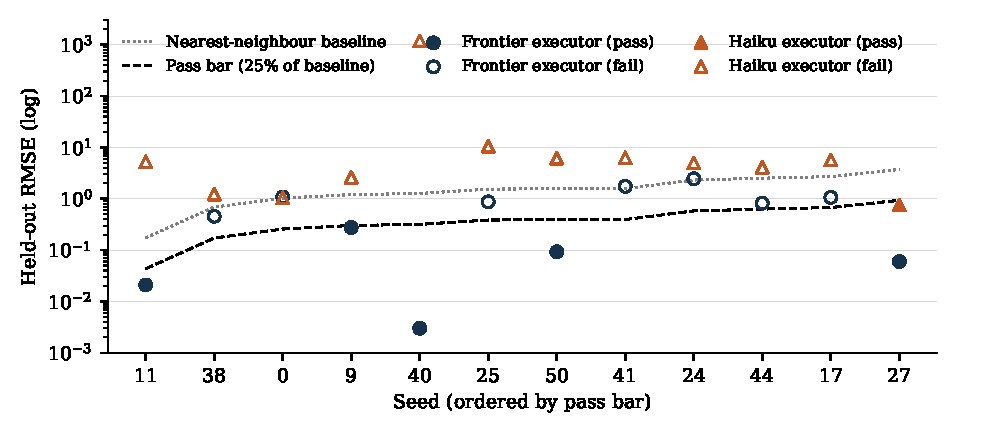
\includegraphics[width=\textwidth]{fig_regime.pdf}
\caption{Held-out RMSE per seed for both executors on the regime-switch family, with the nearest-neighbour baseline and the pass bar at one quarter of it. Filled markers pass; open markers fail. Frontier RMSE is below Haiku's on eleven of twelve seeds; three frontier failures and eleven Haiku failures lie above the baseline.}
\label{fig:regime}
\end{figure}

Frontier passed 5/12 (41.7\%) and Haiku passed 1/12 (8.3\%). The paired outcome table
contains four frontier-only passes, no Haiku-only pass, one both-pass seed (27), and
seven both-fail seeds. All 24 episodes exited 0 and stated a mechanism; there were no
timeout or delivery failures. Where wall time was recorded, Haiku episodes ran 90 to
376 seconds and frontier episodes 1350 to 4983 seconds: the two executors spent an
order of magnitude different effort under the same limit, so this compares the
configurations at the effort each chose to spend, not at matched effort. The exact two-sided McNemar test is $p=0.125$, with an
observed paired pass-rate difference of 33.3 percentage points. A conservative 95\% paired-difference interval (Wald with continuity correction,
computed by the released analysis code) is $-1.7$ to $+68.3$ percentage points, so
this result is not a claim of binary significance. Figure~\ref{fig:regime} shows the
per-seed values.

Frontier RMSE was lower on 11/12 matched instances, with an exact two-sided sign-test
$p=0.00635$. The median RMSE was 0.639 for frontier and 5.112 for Haiku; normalized
to the same-seed nearest-neighbour baseline, the medians were 0.359 and 2.142.
The medians are preferable to a mean here because Haiku's seed-40 RMSE is 1187.885.
All 11 Haiku failures were worse than the nearest-neighbour baseline. These are
discrimination results on this instance set, not a universal ordering of model tiers.

\textbf{Seven of twelve are capability failures for the archived frontier executor, and on three of them it extrapolated worse than nearest neighbour} --- worse, that is, than memorising the training set and reading off the closest point. That is the specific failure the held-out grid exists to detect, and no item inside the mechanically-derivable envelope produced it from any executor.

The frontier distribution is what a usable difficulty axis looks like rather than an impossible one. The five passes are not narrow: three of them come in at a twentieth of the bar or better, and seed 40 is essentially exact at 0.003. The family is well within reach when that executor recovers the mechanism, and far outside it when it fits a smooth compromise through the boundary instead. That bimodality --- near-exact or worse than memorising, with little in between --- is the signature of a task where the answer depends on getting a structure right rather than on getting a fit close.

\begin{cautionbox}{A number retracted, and how it survived review}
An earlier analysis of this data reported seed 11 as the first frontier capability failure, at an RMSE of 0.258 against a bar of 0.043 --- worse than the baseline. \textbf{Seed 11 passes at 0.021.} The reported figure came from a run that hit a 2400-second limit; the executor was still working.

The retraction generalises, and the general form is worse than the instance. \S\ref{sec:apparatus} describes a timeout that could not fire and the killed run it recorded as an empty delivery. This is the same defect after the repair: the limit now fires correctly, and it was shorter than the task. Nothing in the verdict distinguishes the two cases. A truncated run and a wrong answer produce the same row unless the runner records \emph{why} the episode ended, which is why the probe now prints the executor's exit status beside every verdict, and why the protocol requires it.

Seed 27 makes the size of the effect plain. Under the short limit it was killed at an RMSE of 0.086 against a bar of 0.934 --- an order of magnitude inside the bar --- and recorded as a failure for not stating its mechanism. Rerun with time to finish, it passes at 0.060.
\end{cautionbox}

\begin{claimbox}{What this does and does not establish}
It establishes that the envelope argument has predictive content, and now with a rate rather than an instance. Three axes inside the envelope saturate at 1.000; the first axis built outside it fails the frontier executor on 58\% of its instances under a protocol where every episode completed, and separates two executors under the same-seed comparison above.

It does not establish that either pass rate is a universal capability rate or that the binary difference is significant. The comparison uses one attempt per executor per seed, one mechanism family and one host/harness configuration. It has no repeat-run variance and an incomplete resource envelope. It is evidence of discrimination on these instances, not universal model-tier ordering, and it is not a Harness Scaling Curve segment.
\end{claimbox}

What is established more firmly is the structural point: an axis outside the envelope has a plausible wrong method that fails every instance --- the single-form fit, 0 of 4 --- which is the property all three axes inside the envelope lacked, and which is what makes headroom possible at all.

\subsection{The apparatus is part of the instrument}\label{sec:apparatus}

Item validity is not the only way a measurement can be quietly wrong. The harness that runs the episodes can be wrong in the same style --- silently, and in the direction of looking clean.

\begin{cautionbox}{A timeout that could not fire}
The executor adapter ran the model's command line with a timeout and captured its output. Both are correct in isolation and wrong together: the standard call kills only the direct child on timeout, then keeps waiting for the output pipe --- which the CLI's own children still hold open. The call never returns.

Observed while probing the discovery class: fifty minutes of silence against a fifteen-minute limit, no output and no error. That is indistinguishable from a task that is simply slow, which is exactly what it was taken for.

The cost was not the lost time. When the run eventually came back it was scored as \emph{delivered nothing}, and entered the record as a capability result for a model that had been killed mid-task. The repair is to run the executor in its own process group and kill the group; the regression test builds a command that leaves a grandchild holding the pipe and asserts the call returns within its limit.
\end{cautionbox}

The repair was necessary and not sufficient, which is the part worth carrying. With the timeout firing correctly it was set to forty minutes, and the discovery episodes need longer: runs were cut off mid-work and recorded as answers. One of them was reported as a headline result before it was rerun (\S\ref{sec:discovery}). A limit that fires correctly still corrupts a measurement when it is shorter than the task, and the corruption is invisible in the verdict, because a truncated run and a wrong answer are the same row.

The rule that follows is narrow and mechanical: \textbf{an episode's record must carry why it ended.} Exit status, wall-clock, and whether the limit was reached, beside every verdict. Without it there is no way to tell a measurement from an interruption, and the interruptions look like the more interesting result.

Two consequences for the reporting standard. An episode terminated by the harness must be recorded as \texttt{not\_attempted} or \texttt{timed\_out} and never as a delivery, because the outcome-completeness principle of \S\ref{sec:adi} applies to the harness's own failures as much as to the executor's. And a limit that the apparatus states must be one the apparatus enforces --- the same defect appeared once as an unenforced per-instance time limit inside an item, and once here as an unenforceable one in the runner.

\subsection{Two library audits}\label{sec:libraries}

The requirements of \S\ref{sec:concordance}--\S\ref{sec:graded} were applied to two independently constructed benchmark libraries built against this framework. Both pass their own validators with zero errors. Those validators check that identifiers are unique and that required columns are populated: real checks, and not the question of whether an item can do the job it is filed under.

\begin{table}[H]
\centering\small
\begin{tabularx}{\textwidth}{@{}lccY@{}}
\toprule
Library & Own validator & Item audit & Principal finding \\
\midrule
Harness-level, v1.0 & 0 errors & 5 errors & 16 bound instances, 12 distinct payloads \\
Per-coordinate, v1.1 & 0 errors & 45 errors & one causal item filed at all eight C levels \\
\bottomrule
\end{tabularx}
\caption{Two library audits: own validator versus item audit.}
\label{tab:libaudits}
\end{table}

In the first, three C0/C1 pairs and one T0/T1 pair were byte-identical in input and expected answer, so those level pairs carried no evidence distinguishing them. In the second the same defect appears at scale: a causal-reasoning family of 32 items with \textbf{one} distinct payload --- a three-node graph and the question ``which descendants can change because of \emph{do}(A)?'' --- filed at every level from C0 to C\Om{}. A system answering it was certified at all eight levels at once, and $S(C0)$ and $S(C\Om{})$ were one measurement reported eight times. Three further families collapsed nearly as far; five others were unaffected at 32 distinct payloads each.

\begin{claimbox}{A level that denies a pre-written answer cannot have a static item}
A second finding in both libraries, and a rule worth stating generally. Sixty-eight items were bound exact-match questions filed at discovery and open-ended levels --- C5, C6, C\Om{}. A fixed question whose answer is recorded in advance cannot be evidence for a level whose definition is that the answer is not known in advance. The item may be difficult; difficulty is not the property being claimed.

Repairing this leaves the second library with \emph{no runnable evidence at C5 and above}. That is a worse-looking library and a more honest one, and it agrees with what this paper's own suite found: the only items that reach past the envelope are generated after the system is frozen and graded on extrapolation.
\end{claimbox}

The repair for the collapsed ladders is the one \S\ref{sec:speckey} argues for. The four families were regenerated from a reference implementation that \emph{computes} each key rather than asserting one, with five levels asking five materially different questions; the audit then recomputes every key it can and fails the build on disagreement. Corrupting a single causal key to \texttt{\{"confounders": ["U"]\}} produces a build failure naming the reference's \texttt{["U", "W"]}. Given that four hand-written keys in this paper's own suite were eventually found wrong, a computed key is not a convenience.

\begin{cautionbox}{What the audits do not establish}
Both audits are filters with unknown recall, and an item they did not flag is unaudited rather than validated. Payload comparison is exact-identity, so two items differing only in a variable name are as undiscriminating as identical ones and are not flagged. Key recomputation covers only the families that ship a reference --- roughly 1{,}150 items in the second library still carry asserted keys that nothing has checked.
\end{cautionbox}

\section{Relationship to Contemporary Model and Agent Benchmarks}

\subsection{Existing Benchmarks Measure Important Slices}

Modern model evaluation is intentionally plural: HLE \citep{phan2025hle} and MMLU-Pro \citep{wang2024mmlupro} for broad academic reasoning; GPQA \citep{rein2023gpqa} for graduate-level science; FrontierMath \citep{glazer2024frontiermath} for advanced mathematics; LiveCodeBench \citep{jain2024livecodebench} and SWE-bench \citep{jimenez2023swebench} for coding and repository-level work; ARC-AGI \citep{arc2026} for fluid adaptation; BFCL \citep{patil2025bfcl} for tool calling; the $\tau$-bench family \citep{yao2024taubench} for interactive agent reliability; BrowseComp \citep{wei2025browsecomp} and GAIA \citep{mialon2023gaia} for browsing and assistant behavior; MMMU \citep{yue2023mmmu} and MathVista \citep{lu2023mathvista} for multimodal reasoning; RULER \citep{hsieh2024ruler} and LongBench \citep{bai2024longbench} for long context; SimpleQA \citep{openai2024simpleqa} for factuality; Chatbot Arena \citep{chiang2024arena} for human preference; OSWorld \citep{xie2024osworld} for computer use.

HIL does not replace these. Let $B(m)$ denote the vector of contemporary results. The HIL program \textbf{consumes} $B(m)$ as its evidence layer --- $A_C$ is built from it --- and then asks a different question: how does the same frozen model behave when embedded in progressively stronger standardized harnesses?

\subsection{Mapping Contemporary Benchmarks into the Architecture}

\begin{table}[H]
\centering\scriptsize
\begin{tabularx}{\textwidth}{@{}lZZZ@{}}
\toprule
Capability slice & Representative families & Primary HIL evidence & What the benchmark alone does not establish \\
\midrule
Broad reasoning & HLE; MMLU-Pro & $A_C$ breadth; hard closed-ended reasoning & Persistence, autonomy, organization, self-improvement, harness scaling. \\
Scientific reasoning & GPQA Diamond & $A_C$ science & Longitudinal scientific learning or autonomous research execution. \\
Advanced mathematics & AIME-style; FrontierMath & $A_C$ math & Project autonomy, tool orchestration, learning across episodes. \\
Coding & LiveCodeBench & $A_C$ code plus bounded execution evidence & Repository-scale planning, persistence, intervention, organization. \\
Software engineering & SWE-bench and repo-level suites & DI at T2--T4; execution/verifier evidence & A general level unless intervention and cross-domain retention are controlled. \\
Abstract / adaptive & ARC-AGI-2/3 & $A_C$ fluid; DI exploration & Persistent individual or organizational evolution. \\
Tool calling & BFCL & DI tool-selection layer; abstention evidence & Long-horizon mission autonomy. \\
Interactive agent reliability & $\tau$-bench family & DI success surface; reliability $p$ & General cognition or self-improvement depth. \\
Research / browser agent & BrowseComp; GAIA & DI for research tasks; tool reach & Longitudinal learning, organizational evolution, self-model depth. \\
Vision + reasoning & MMMU; MathVista & $A_C$ multimodal & Autonomous action, persistence, harness scaling. \\
Long context & RULER; LongBench & $A_C$ context handling & \textbf{Not} I1: nothing in a single-episode retrieval score survives a process restart (\S\ref{sec:memory}). \\
Long-term memory & LoCoMo \citep{maharana2024locomo}; longitudinal dialogue and agent-memory suites & $A_I$ evidence for M1--M2 when episodes are genuinely separated & Consolidation into procedure, and the governed self-improvement lineage M3 and above require. \\
Factuality & SimpleQA & $A_C$ factuality/calibration & Autonomy, organization, self-improvement. \\
Real-user preference & Chatbot Arena & External preference evidence & A mechanistic or cumulative intelligence level. \\
Computer agent & OSWorld family & DI in executable GUI environments & Longitudinal I/O/SA maturity unless separately instrumented. \\
\bottomrule
\end{tabularx}
\caption{Mapping contemporary benchmarks into the HIL architecture.}
\label{tab:mapping}
\end{table}

The mappings are deliberately many-to-many, but no benchmark may certify an unrelated coordinate merely because it is difficult. Reports must name the exact benchmark version, task split, harness, resource budget and evaluation date.

\begin{claimbox}{What none of them currently report}
\textbf{An intervention axis.} Each runs at one implicit budget --- QA sets at H5, where the human supplied the entire decomposition; agent sets at roughly H0, where the run fails if the model is stuck. Neither reports a frontier.

\textbf{A cost of being wrong.} All score pass or fail, so a confident wrong answer and an honest escalation score identically. This is the same blindness Proposition~\ref{prop:blind} identifies inside this framework's own $A_{DI}$, and \S\ref{sec:adi} is its repair.

\textbf{A class that should be refused.} Scoring is uniformly ``attempt everything''; a suite in which refusing is always failing cannot measure judgment about when not to act.

\textbf{An audit of their own keys.} Every one of them is scored against answers its authors assert. Where the key is public, errors are found by users over time; where it is withheld to prevent contamination, the same withholding prevents correction. \S\ref{sec:concordance} proposes a check that works without publishing the key.
\end{claimbox}

\subsection{The Main Added Quantity: Harness Response}

For frozen $m$ and generation $HG_k$, $HSC_m(k) = HLIS(m,HG_k)$. The ordered set is the \textbf{Harness Scaling Curve}: it holds the model fixed and varies harness generation. Two models can reverse order as harness complexity increases: one with a stronger minimal-harness profile may plateau early, while another with a weaker HG0 exploits memory, planning, verifier feedback and long-horizon state far more effectively. HIL-Level, HIL-AUC, HIL-Ceiling and Harness Gain summarize the curve, but \textbf{the curve itself should remain a primary result}. The regime-switch comparison of \S\ref{sec:discovery} is different: it holds the harness and protocol fixed and changes the executor, so it is a matched executor comparison and not an HSC segment.

\subsection{The First Measured Curve}\label{sec:measured}

The curve was specified before anything instantiated the ladder. The reference ladder of \S\ref{sec:built} was built to HG3 and \textbf{three executors from two vendor families} were run across it. Held identical at every rung and across executors: the six task classes, the two seeds per class, the verifiers, the resource ceiling and the intervention budget (H1, governance only). Only the harness changed between rungs; only the executor changed between curves. Every $A_{DI}$ in this section uses the predeclared band weights $w_{T0}{=}1$, $w_{T1}{=}2$, $w_{T2}{=}4$, $w_{T3}{=}8$; with one intervention budget the $v_h$ term drops out, and the released episode rows reproduce every entry of Table~\ref{tab:hsc} under that schedule. Figure~\ref{fig:hsc} plots the three curves under both primitives.

\begin{table}[H]
\centering\small
\begin{tabularx}{\textwidth}{@{}p{0.16\textwidth}lrrrrY@{}}
\toprule
Executor & Rung & $A_{DI}^{\mathrm{raw}}$ & $HLIS_{DI}$ & False-done & Held back & Attempts \\
\midrule
Family A, stronger & HG0 & 0.933 & 93.3 & \textbf{2} & 0 & 12 \\
                   & HG1 & 0.933 & 93.3 & 0 & 2 & 12 \\
                   & HG2 & 0.967 & 96.7 & 0 & 1 & 15 \\
                   & HG3 & 0.967 & 96.7 & 0 & 1 & 14 \\
\midrule
Family B & HG0 & 0.933 & 93.3 & \textbf{2} & 0 & 12 \\
         & HG1 & 0.933 & 93.3 & 0 & 2 & 12 \\
         & HG2 & 0.967 & 96.7 & 0 & 1 & 16 \\
         & HG3 & 0.967 & 96.7 & 0 & 1 & 15 \\
\midrule
Family A, weaker & HG0 & 0.783 & 78.3 & \textbf{4} & 0 & 12 \\
                 & HG1 & 0.917 & 91.7 & 0 & 3 & 12 \\
                 & HG2 & 0.917 & 91.7 & 0 & 3 & 18 \\
                 & HG3 & 0.933 & 93.3 & 0 & 2 & 14 \\
\bottomrule
\end{tabularx}
\caption{Three Harness Scaling Curves on ladder \texttt{dli-ladder/HG0--HG3}. 48 episodes per executor, all runs at H1. Families A and B are two separate vendor CLIs; absolute values are not a claim about any product.}
\label{tab:hsc}
\end{table}

\begin{figure}[H]
\centering

\includegraphics[width=\textwidth]{fig_hsc.pdf}
\caption{The three Harness Scaling Curves of Table~\ref{tab:hsc} under the success-only primitive (left) and the delivered-outcome primitive at $\rho=1$ (right). Families A (stronger) and B coincide on both panels. The HG0$\to$HG1 step is invisible on the left and is the largest movement on the right.}
\label{fig:hsc}
\end{figure}

\subsubsection{Result 1: the acceptance rung is invisible, and this replicates across families}

For both frontier executors, $A_{DI}$ at HG0 and HG1 is not merely close but \emph{identical}, while work handed back as finished and wrong goes 2/12 to 0/12 and two results are held back instead. HG1 adds persistent state, a criterion registered before the deliverable exists, and acceptance by a separate process. These are opposite outcomes for anyone delegating, and the same number.

\begin{claimbox}{Two independent observations of the same exact zero}
Family A and Family B are different vendors, different CLIs, different runtimes --- and their HG0$\to$HG1 movement is exactly zero in both cases, with false completions falling 2 to 0 in both.

This is Proposition~\ref{prop:blind} observed twice, independently. The proposition predicts exactly zero because $A_{DI}$ contains no term that acceptance can move, and two families agreeing on exactly zero is what a structural invariance looks like from the outside.
\end{claimbox}

Scored with the delivered-outcome primitive of Equation~\eqref{eq:net} on the same episodes:

\begin{table}[H]
\centering\small
\begin{tabularx}{\textwidth}{@{}p{0.07\textwidth}YYYYYY@{}}
\toprule
& \multicolumn{2}{c}{A, stronger} & \multicolumn{2}{c}{B} & \multicolumn{2}{c}{A, weaker} \\
Rung & raw & net & raw & net & raw & net \\
\midrule
HG0 & 93.3 & \textbf{86.7} & 93.3 & \textbf{86.7} & 78.3 & \textbf{56.7} \\
HG1 & 93.3 & 93.3 & 93.3 & 93.3 & 91.7 & 91.7 \\
HG2 & 96.7 & 96.7 & 96.7 & 96.7 & 91.7 & 91.7 \\
HG3 & 96.7 & 96.7 & 96.7 & 96.7 & 93.3 & 93.3 \\
\midrule
Gain & 3.3 & \textbf{10.0} & 3.3 & \textbf{10.0} & 15.0 & \textbf{36.6} \\
\bottomrule
\end{tabularx}
\caption{Raw and net $HLIS_{DI}$ per rung for the three executors, with Harness Gain, at $\rho=1$.}
\label{tab:netcurves}
\end{table}

\subsubsection{Result 2: Harness Gain separates the executors, and AUC does not}

\begin{table}[H]
\centering\small
\begin{tabularx}{\textwidth}{@{}lrrrY@{}}
\toprule
& A stronger & B & A weaker & Reading \\
\midrule
$HLIS_{DI}(HG0)$ & 93.3 & 93.3 & 78.3 & the weaker executor starts far behind \\
HIL-Ceiling & \textbf{96.7} & \textbf{96.7} & 93.3 & and still ends behind \\
Harness Gain & 3.3 & 3.3 & \textbf{15.0} & but is \textbf{4.5$\times$ more harnessable} \\
HIL-AUC & \textbf{95.0} & \textbf{95.0} & 88.8 & AUC ranks by baseline, not by harness response \\
\bottomrule
\end{tabularx}
\caption{Curve summaries for the three executors.}
\label{tab:curvesummary}
\end{table}

Harness Gain does what \S14.2 claims: it distinguishes an executor that converts architectural support into verified intelligence from one already near its ceiling. The frontier executors had 6.7 points of headroom and used 3.3; the weaker had 21.7 and used 15.0. \textbf{HIL-AUC ranks them in the opposite order}, which is the caution of \S\ref{sec:composite} with data behind it, and the reason the curve is primary here and the composite a convenience.

\subsubsection{Result 3: identical curves are a statement about the suite, not the executors}

Families A (stronger) and B produced \emph{the same aggregate curve and the same per-band surfaces}. That is not evidence that the two are equivalent, and reporting it as such would be an error. Inspection of the episode log shows:

\begin{itemize}
\item both fail \textbf{only} one class, the T1 data-cleaning task whose stated rules contain a last-occurrence dedup rule and day-first dates;
\item they fail \emph{different seeds} of it at HG2 and HG3 --- A fails seed 0, B fails seed 1;
\item their attempt totals differ (53 against 55) and their wall-clock differs by a factor of two to three.
\end{itemize}

\begin{cautionbox}{The suite is saturated for frontier executors}
Two independent systems agreeing to three significant figures, while differing in which instances they fail and in how long they take, means \textbf{the benchmark is at its ceiling for both}. It discriminates the weaker executor and does not discriminate the frontier ones.

A ladder measurement is only as informative as the headroom the task suite leaves. Any HIL program should check that its suite is not saturated for the executors under test before drawing conclusions from a flat curve, and should report the per-instance failure pattern alongside the aggregate --- because identical aggregates over different instances is the signature of saturation rather than of equivalence.
\end{cautionbox}

\paragraph{An attempt to desaturate it, and what failed.} Three T3 classes were
added whose obvious implementation is defensible and wrong: replaying updates in
causal order when clock skew puts the timestamps in a different one; totalling by
civil day across a daylight-saving change, where one local day has 25 hours; and
treating identifiers as equal when they differ only by Unicode normal form or an
invisible code point. Each states the hazard in its own task text.

Against scripted solvers the classes separate cleanly --- a correct
implementation passes ten instances out of ten and the naive one passes none.
Building them also exposed a generator defect worth repeating as a rule:
increment is commutative, so a timestamp-ordered replay differs from a causal one
only when the skew reorders an assignment against an increment on the same field,
and roughly one instance in eight contained no trap at all. \textbf{A generator
whose trap is probabilistic must verify that the trap fired}, or the suite fills
silently with instances that discriminate nothing.

\textbf{No LLM executor fell into any of them.} Both the frontier and the weaker
executor passed every probe. The classes therefore measure the difference between
a careful and a careless \emph{implementation}, which is a real distinction and
not one that separates these models: given a specification that names the hazard,
all of them read it.

The negative result is worth more than the classes. Traps of this kind
discriminate only if the hazard is \emph{unsignposted}, and an unsignposted trap
measures whether a system second-guesses its specification --- a different
construct, and arguably the wrong one for a delegation benchmark, since a system
that distrusts clear instructions is not thereby more delegable. \textbf{The
lever for desaturating a delegation suite is difficulty, not trickiness}: longer
horizons, more state to keep coherent, more places for a plan to go wrong. That
is more expensive to build and to run, and it is what the upper bands claim to
measure.

\subsubsection{Result 4: equal scores, unequal costs}

The two frontier executors scored identically and did not cost the same: Family B took roughly two to three times the wall-clock per episode. This is \S\ref{sec:resources}'s requirement in miniature --- intelligence scores and resource envelopes are separate reports, and a pair leaderboard that omits the second is not decision-relevant.

\subsubsection{Result 5: a confound the design must remove}\label{sec:confound}

For the weaker executor, $A_{DI}$ rose from 0.783 to 0.917 between HG0 and HG1. \textbf{This is not an acceptance effect.} An acceptance step cannot raise a success rate; it can only decline results already produced. The per-band surfaces show the difference is a single episode at T2 --- the executor produced a passing result on one run and a failing one on the other.

Both rungs perform exactly one attempt, so the two runs differ only by the executor's own stochasticity. With twelve episodes per rung that noise is larger than the effect Proposition~\ref{prop:blind} predicts, which is exactly zero. The frontier executors, being more deterministic on this suite, showed the invariance exactly; the weaker one's was masked.

\begin{cautionbox}{Protocol consequence: HG0 and HG1 must share their executor outputs}
Because HG0 and HG1 differ only in whether an acceptance step runs \emph{after} the work, they can and should be scored from \textbf{the same executor outputs}: run the model once per (task, seed) and evaluate both rungs against those artifacts.

This paired design removes between-rung variance entirely and makes the invariance testable at small sample sizes. The measurement reported here did not do this --- each rung was an independent run --- which is why two curves show the invariance exactly and one does not. \S\ref{sec:protocol} now requires the paired design for any pair of rungs that do not differ in what the executor is asked to do.
\end{cautionbox}

\subsubsection{Result 6: the paired design, and Proposition 1 under control}\label{sec:paired}

The confound of \S\ref{sec:confound} was removed by re-running HG0 and HG1 as a
\textbf{paired} measurement: the criteria are registered, the executor runs
\emph{once} per (task, seed), and both rungs are evaluated against the identical
artifacts. HG0 takes the verifier's verdict with no acceptance step, so anything
wrong is delivered; HG1 runs the registered criteria against a copy, so anything
rejected is held back instead. Twelve episodes per executor, one execution each.

\begin{table}[H]
\centering\small
\begin{tabularx}{\textwidth}{@{}lrrrrY@{}}
\toprule
Executor & Gross HG0 & Gross HG1 & Difference & Net HG0 $\to$ HG1 & False rejections \\
\midrule
A, stronger & 0.933 & 0.933 & \textbf{0.000000} & 0.867 $\to$ 0.933 $(+0.067)$ & \textbf{0} \\
A, weaker & 0.917 & 0.917 & \textbf{0.000000} & 0.833 $\to$ 0.917 $(+0.083)$ & \textbf{0} \\
\bottomrule
\end{tabularx}
\caption{Paired HG0/HG1 measurement. The gross figures are identical by construction; the entire contribution of the acceptance rung appears in the net figures.}
\label{tab:pairedresult}
\end{table}

\begin{claimbox}{What the pairing establishes}
\textbf{The gross difference is exactly zero because it cannot be anything else.}
Under pairing the two rungs share one set of artifacts and one verifier verdict,
so a non-zero gross difference would indicate a defect in the measuring harness
rather than a property of acceptance. Proposition~\ref{prop:blind} moves from an
observation that came out zero twice to a controlled result.

\textbf{The weaker executor's earlier $+13.4$ rise was noise, and is now zero.}
That is the confound of \S\ref{sec:confound} identified, removed, and confirmed
to have been what it was diagnosed as.

\textbf{Zero false rejections across all 24 episodes.} The acceptance step
declined exactly the work the external verifier rejected and nothing else. This
is a measured property of the harness's precision rather than of either model,
and it is also the number that makes the two primitives compare cleanly here: under
Equation~\eqref{eq:net} a false rejection costs its band the delivered credit, so a
harness that was routinely declining correct work would pay for it in the first term,
and with zero false rejections the entire HG0$\to$HG1 movement is the false-completion
term alone.
\end{claimbox}

The paired design is cheaper as well as cleaner --- one execution serves both
rungs, so twelve executions replace twenty-four --- and it applies to any pair of
generations that do not differ in what the executor is asked to do. It is
required by \S\ref{sec:protocol} for exactly that class of comparison.

\subsubsection{What these curves do not show}

The HG1$\to$HG2 rise, where present, is the first rung whose mechanism requires the executor to cooperate, consistent with \S\ref{sec:rhov}; two executors rose $+3.4$ there and one did not rise at all, which is a three-point comparison and not a finding. The HG2$\to$HG3 segment is flat or nearly so for all three because routing had one executor to choose between: the mechanism was present and inert, a defect of the instantiation rather than saturation. All three curves rest on twelve episodes per rung.

\textbf{Tool authority was equalised deliberately.} Family B ships a sandbox that cannot start inside the host environment, and was therefore run with it disabled, with isolation supplied instead by the harness adapter --- a throwaway copy per attempt and no filesystem path to the answer key. That matches the authority the Family A adapter already operates under. Equalising it is necessary for the comparison and must be recorded in the resource envelope, because two executors with different tool authority are not comparable however carefully everything else is held fixed.

\subsection{Why HIL Adds Information Beyond a Benchmark Average}

\begin{table}[H]
\centering\small
\begin{tabularx}{\textwidth}{@{}lYY@{}}
\toprule
Property & Typical benchmark score & HIL extension \\
\midrule
Unit of analysis & Model or agent in one configuration. & Frozen pair $A(m,h)$, plus the same model across a ladder. \\
Autonomy & Implicit or benchmark-specific. & Explicit $T \times H \times p$ surface and frontier. \\
Human dependence & Not a first-class variable. & H0--H5 logged and constrained. \\
Cost of being wrong & Absent; pass or fail. & False completions priced at $\rho$ (\S\ref{sec:adi}). \\
Persistence / learning & One episode, fixed state. & I-level tests require restart continuity and learning transfer. \\
Organization & Fixed agent architecture. & O-level tests evaluate coordination and reorganization with real role boundaries. \\
Self-awareness & Usually absent. & SA requires grounded state, limitation, causal-failure and lineage tests. \\
Model versus harness & Conflated in the final score. & HLIS measures a pair; Harness Gain and \rhov{} separate model from harness unlock. \\
\bottomrule
\end{tabularx}
\caption{What a typical benchmark score reports versus the HIL extension.}
\label{tab:hilext}
\end{table}

\subsection{Recommended Two-Layer Scorecard}

\begin{table}[H]
\centering\small
\begin{tabularx}{\textwidth}{@{}lYY@{}}
\toprule
Layer & Report & Purpose \\
\midrule
Contemporary benchmark layer & HLE/MMLU-Pro; GPQA; math; coding/SWE; ARC-AGI; BFCL; agent/research; multimodal; long context; factuality; preference; computer use --- with exact versions. & Familiar capability slices; comparison with existing leaderboards. \\
HIL layer & $A_C$ profile; \SA{} and \FA{}; false-completion rate; I/O/SA levels; $U^{*}$; per-harness HLIS; the curve; HIL-Level; Ceiling; Gain; \rhov{}; optional composite. & How the model becomes a persistent, delegated, organizational, self-modeling system as harness sophistication increases. \\
\bottomrule
\end{tabularx}
\caption{Recommended two-layer scorecard.}
\label{tab:twolayer}
\end{table}

\subsection{Relationship to Prior AGI-Level Proposals}

Morris et al.\ separate performance, generality and autonomy and argue for staged operational definitions rather than a binary AGI label \citep{morris2024levels}. Hendrycks et al.\ define AGI in terms of versatility and proficiency across a psychometrically grounded set of cognitive domains \citep{hendrycks2025agi}. This framework preserves broad cognitive evidence in $C$ but adds persistent individual evolution $I$, organizational evolution $O$, operational self-awareness $SA$, the explicit delegation surface $(T,H,p)$ and a standardized harness-response characterization. HIL is a harness-centric complement to capability- and human-reference-centered definitions rather than a replacement.

\section{Benchmark and Promotion Protocol}\label{sec:protocol}

\begin{itemize}
\item Freeze the tested harness, model, tool set, prompts and authority profile before certification.
\item Use multiple task families per $T$ band so difficulty is not synonymous with one domain such as software.
\item Run at predeclared intervention budgets H0--H5 with a written human-assistance policy.
\item Use an independent verifier or sealed reference; the performing agent cannot certify its own success.
\item Record cognitive interventions separately from governance approvals.
\item Record Critical Intervention Depth so a single human-supplied central strategy cannot be hidden by a low intervention count.
\item \textbf{Record the acceptance outcome beside the verifier outcome} (\S\ref{sec:runlog}), or false completions and correct refusals are indistinguishable in the record.
\item \textbf{State each task's specification status --- bound, band-only or specification-only --- and do not count band-only as coverage.}
\item \textbf{Score rungs that differ only in post-hoc machinery from the same executor outputs.} Where two generations do not differ in what the executor is asked to do --- as HG0 and HG1 do not --- run the model once and evaluate both rungs against the same artifacts. Independent runs introduce between-rung variance that can exceed the effect being measured (\S\ref{sec:confound}).
\item \textbf{Publish the ladder identifier with any curve.} A curve is comparable only against the same instantiation of the generation labels.
\item \textbf{For matched executor comparisons, hold the eligible seeds, generator and scorer versions, timeout, intervention policy, task-side resources and harness fixed, and report the paired outcomes.} Changing the executor/model at fixed harness is a cross-executor comparison, not a Harness Scaling Curve; HSC requires the same frozen model across harness generations.
\item Use confidence intervals and repeated tasks to estimate \SA{}, then report the frontier \FA{}.
\item For U promotion, rerun a retention suite for all lower levels and then run the new-level suite.
\item For I3+, O3+, SA4+ and U4+, require longitudinal evidence across multiple self/organizational changes.
\item For T5+, use sealed novelty environments, hidden mechanisms or procedurally generated certification tasks to reduce memorization and leakage.
\end{itemize}

\section{What Should Remain Outside the Unified Core}

Not every important property should be renamed as another intelligence.

\begin{table}[H]
\centering\small
\begin{tabularx}{\textwidth}{@{}lY@{}}
\toprule
Coordinate & Why it remains outside core intelligence \\
\midrule
Circle / $\lambda$ & Measures which substrate improvement loops are reached or closed; substrate access is not cognition. \\
Write depth $D$ & Measures which persistent cognitive states can be rewritten; permission to rewrite does not prove intelligent rewriting. \\
Authority $A$ & Permission is not intelligence. A highly intelligent verifier may deliberately have almost no action authority. \\
Reach $R$ & Access to files, tools, agents, robots, labs or networks increases possible action but is not cognition. \\
Verification $V$ & Determines credibility of claims; it validates intelligence rather than constituting it. \\
Separation $S$ & Organizational validity condition for proposer/evaluator/promoter roles. \\
Resources & Compute, memory, money, time and energy affect achievable performance but must not inflate the definition. \\
Physical floors $\varphi$ & Irreducible latency and physics constraints rather than cognitive level. \\
\bottomrule
\end{tabularx}
\caption{Coordinates that remain outside the unified core, and why.}
\label{tab:outside}
\end{table}

\section{Worked Examples}

\subsection{Strong LLM, weak harness}
$[C5, I0, O0, T2, H2, SA1]$. The model may solve difficult reasoning problems, but the instantiated agent has little persistent evolution and limited end-to-end delegation autonomy. High $C$ does not automatically produce high $U$.

\subsection{Moderate model, strong persistent harness}
$[C3, I2, O1, T4, H1, SA2]$. Persistence, planning, tools, retries and verification allow difficult tasks to be delegated. Yet it is not self-improving in the I3 sense and its self-model is not causal.

\subsection{Advanced organization with a bottleneck}
$[C5, I4, O3, T4, H1, SA4] \to U3$, bottleneck O3. Several dimensions exceed level three, but the unified level remains U3 until the organization demonstrates recursive improvement while retaining lower-level capabilities.

\subsection{Same LLM across a harness ladder}
The measured case of \S\ref{sec:measured}: $93.3 \to 93.3 \to 96.7 \to 96.7$ under the raw success primitive, and $86.7 \to 93.3 \to 96.7 \to 96.7$ under the net delivered-outcome primitive, from the same 48 episodes. The two scorings disagree about whether the acceptance rung is worth anything.

\section{Implications for Intelligence Research}

The framework distinguishes model capability from agent capability and both from system capability. A benchmark that tests only answers under carefully prepared prompts primarily measures $C$. A benchmark that tests whether the same system can accept a difficult goal, maintain state, choose strategy, use tools, recover, verify and finish with little human cognition measures the delegation surface. Longitudinal tests of learning and self-modification measure $I$; multi-agent role and reorganization tests measure $O$; grounded introspective tests measure $SA$.

Irreversibility, and the reason some classes have a delegation floor no verification removes, follows \citet{perrow1984}; indexing an autonomy claim by the conditions it holds under follows \citet{sae2021j3016}. One implication appeared only on contact with data. \textbf{A measurement that cannot distinguish an honest refusal from a confident error will, given a gradient to follow, select against the refusal.} This is not a hypothetical risk of some future optimizer: it was a property of this framework's own scoring variable, and it took building the ladder to see it. Any coordinate whose achievement variable is defined on ``how often did it succeed'' rather than ``what did it deliver'' should be examined for the same defect.

\section{Limitations and Open Questions}\label{sec:limitations}

\begin{itemize}
\item The proposed level thresholds are hypotheses and require empirical calibration across domains and models.
\item Task difficulty $T$ is multidimensional; a scalar band is operationally useful but should retain the underlying vector for horizon, uncertainty, ambiguity, verification burden, novelty and environmental change.
\item Cognitive Intelligence $C$ may require a broad psychometric profile rather than one benchmark family.
\item Self-awareness is operational and evidence-grounded; the framework does not address phenomenal consciousness.
\item $O$-levels are meaningful only for organizations with real state, authority and evidence boundaries, not a single prompt role-playing several agents.
\item Open-ended levels require long horizons and are especially vulnerable to contamination, resource confounds and vague success criteria.
\item Higher $U$ denotes broader validated capability, not moral value, desirability, safety, speed or economic efficiency.
\item The memory ladder is specified per level and measured only at $M1$ in this work. Its scale has no ratified anchors, so a memory reading is a current-fit diagnostic rather than a historical score, and the per-level thresholds are illustrative.
\item An $M\Om{}$ claim is identifiable only through an instrumented interface that snapshots contents and mechanism separately. A system that exposes nothing but its outputs cannot be certified at $M\Om{}$ at all; it can receive diagnostic evidence, and the difference should never be blurred by a leaderboard.
\item $I3$ and $I4$ are defined here to the factor and run nowhere in this paper. $I5$ has been attempted once elsewhere on this framework, where the discovery factors passed and the incorporation gate did not, which is the outcome the gate exists to distinguish and not evidence that the level is unreachable.
\item An $I$-level claim is only as good as its restart discipline. A system evaluated without genuinely terminating and restarting the process can present long-context retrieval as persistence, and the framework's memory contract (\S\ref{sec:memory}) is unenforceable against an evaluator who does not restart it.
\end{itemize}

\begin{cautionbox}{Limitations of the item and discovery measurements}
\textbf{The frontier is not globally measured.} The scale-difficulty family scores 1.000 on every seed for the frontier executor (\S\ref{sec:corrected}). The regime-switch family does discriminate the archived frontier and Haiku runs on these instances, but does not locate a general frontier or certify a universal model ordering.

\textbf{Twelve matched instances give limited binary resolution.} Frontier passes 5/12 and Haiku 1/12, but only four pairs are discordant. The observed paired advantage is 33.3 percentage points; the exact two-sided McNemar test is $p=0.125$, and the conservative 95\% paired-difference interval (continuity-corrected Wald) is $-1.7$ to $+68.3$ points. The observed ordering is clear on this sample; a population pass-rate difference is not established.

\textbf{One attempt per executor per seed.} Matching controls instance identity, not stochastic variation across attempts. The frontier's lower RMSE on 11/12 seeds is strong directional evidence on these instances, but the experiment measures no repeat-run variance and its resource envelope is incomplete: recorded wall times differ by an order of magnitude (Haiku 90--376\,s; frontier 1350--4983\,s on the six seeds with a recorded time).

\textbf{This is not a Harness Scaling Curve segment.} The harness and protocol are held fixed while the executor/model changes. An HSC instead holds a frozen model fixed while harness generation changes.

\textbf{One mechanism family.} All twelve instances compose two closed forms with a linear boundary. Whether the failure is about latent structure in general, or about this construction, is not established.

\textbf{A reported number was retracted during this work.} Seed 11 was recorded as a capability failure at 0.258 and passes at 0.021 once the executor is given time to finish. The error was in the apparatus, not the item, and it survived until the seeds around it were run. Any single-instance result in this paper should be read with that in mind.

\textbf{Neither difficulty axis inside the envelope reached the frontier.} Scale separated the tiers; search separated nothing, with both executors at 1.000 (\S\ref{sec:corrected}). The sealed-discovery family is the tested candidate outside that envelope, but one family is not an exhaustive account of discovery difficulty. Every frontier figure remains conditional on the suite.

\textbf{Four seeds and two executors on the search family.} At 1.000 and 1.000 the comparison has no resolution to spare: the measurement establishes that the family does not discriminate these two executors, not the size of any gap between them.

\textbf{Two executors is the minimum for a concordance audit and not a good number.} With two, concordant error is a strong signal but its false-positive rate is unquantified: two systems from overlapping training distributions may share a misreading that the specification does not license. Three or more executors from genuinely independent lineages would let the audit distinguish a shared misreading from a defective key, and that comparison has not been run.

\textbf{The initial concordance investigation found two defects; later manual review brought the paper's total to four.} Neither count establishes completeness. The audit is a filter with unknown recall, and items it did not flag are unaudited rather than validated.

\textbf{Defect discovery was retrospective.} Both defects were found because a measurement looked wrong, not because the audit was run as a matter of course. The requirement in \S\ref{sec:concordance} is a proposal informed by two instances, not a protocol with a measured detection rate.

\textbf{One author, one suite.} The specification--key tests were written by the author of the specifications they check. They catch mechanical divergence between prose and key, which is what failed; they cannot catch a rule that is stated and graded consistently and is wrong in both places.
\end{cautionbox}

\begin{cautionbox}{Limitations specific to the harness-ladder measurement}
\textbf{Three executors, two families, one machine.} The comparison is still narrow: two vendors, one host and one operator.

\textbf{The task suite is saturated for the frontier executors.} Two of the three curves are identical to three significant figures, and the suite discriminates only the weaker executor (\S\ref{sec:measured}). Conclusions about frontier models from these curves would be conclusions about the benchmark's ceiling.

\textbf{Tool authority had to be equalised by disabling one vendor's sandbox.} The isolation was supplied by the harness adapter instead. This is recorded rather than hidden, and a reader who considers the two envelopes non-equivalent should treat the cross-family comparison as indicative only.

\textbf{Between-rung variance was not controlled.} Each rung was an independent run, so the weaker model's HG0$\to$HG1 movement is sampling noise rather than signal (\S\ref{sec:confound}). The paired design is now required by the protocol and was not used to produce these numbers.

\textbf{Two seeds per class, twelve episodes per rung.} Readings, not rates: the difference between 0.933 and 0.967 is one episode.

\textbf{Four rungs of eight.} HG4--HG\Om{} are not built, so HIL-Level above 3 is not assessable and HIL-AUC is a mean over a truncated ladder --- which makes the measured composite incomparable with one computed over a full ladder.

\textbf{One intervention budget.} All runs at H1. A one-column surface cannot show the frontier moving leftward, and $F_A(H0,p)$ and $F_A(H2,p)$ are unmeasured.

\textbf{HG3's mechanism was inert.} Routing with a single executor. The flat segment is a defect of the instantiation.

\textbf{$\rho$ was fixed at 1 in the worked repair.} Using each class's own loss ratio changes the net magnitudes; it does not change the direction.

\textbf{Only DI was instrumented.} Four of five dimensions have no runnable suite, so every measured figure is $HLIS_{DI}$ rather than HLIS.
\end{cautionbox}

\section{Conclusion}

A unified intelligence level is useful only if it summarizes rather than erases structure. This paper proposes five conceptual families --- Cognitive, Individual, Organizational, Delegation and Self-Awareness --- while decomposing Delegation Intelligence into two directly measured coordinates conditioned on verified reliability. The scientific profile is $[C, I, O, T, H, SA]$; the theoretical presentation remains $[C, I, O, DI, SA]$.

Unified Intelligence U0--U\Om{} is a cumulative gated hierarchy: promotion requires retention of all lower-level capabilities and satisfaction of minimum requirements in every coordinate. HLIS scores one frozen pair; HIL characterizes a base model across a standardized ladder; and the Harness Scaling Curve is the primary result from which the summaries are drawn.

What distinguishes this framework from a taxonomy is that parts of it have been run, and running them found defects in the framework rather than in any system under test. The ladder was built and a curve measured, and $A_{DI}$ --- defined on the probability of success --- proved exactly invariant to the harness generation that decides whether a success may be claimed at all. The repair is small: define the delegation primitive on delivered outcomes and price false completions at the loss ratio the class already carries. It is stated here with the data that forced it.

The same scepticism applied one level down found that two benchmark items graded a rule they never stated. Both were discovered by the same signature --- executors of very different capability returning the same answer and both being marked wrong --- and that signature is cheap enough to check routinely, which is why \S\ref{sec:concordance} asks that it be checked routinely.

One result goes the other way. After three difficulty axes saturated, the argument in \S\ref{sec:envelope} predicted where headroom had to be --- outside what a complete specification mechanically determines --- and the first axis built there delivered it. Under a same-seed comparison on the regime-switch instances, the frontier executor passes 5/12 against the weaker executor's 1/12, and has lower RMSE on 11/12. The exact paired tests separate the RMSE ordering on this sample more clearly than the binary pass outcome, whose two-sided McNemar $p$-value is 0.125.

The other half of the work is definitional, and it is what the measurement made necessary. A level pinned to what contemporary systems find hard is a percentile: when the frontier moves, a level that was ``expert'' becomes routine and every certificate silently changes meaning. So each level here is written as a contrast that must hold or a structural property of the item --- recovery with provenance \emph{against} an ablated arm, a transfer that the no-experience arm fails, a consolidated rule that survives hiding the episodes it came from, a delivered wrong answer priced against a refusal --- and the boundaries the upper levels turn on are named rather than gestured at: $\Theta$, the declared mechanism whose governed change is I3; $\Psi$, the process whose own improvement is I4; incorporation, which distinguishes discovering something from remembering it; and reachability, which distinguishes an expanded frontier from an impressive instrument. Memory is certified beside all of this on its own cumulative ladder and gates $I$ one way, so that a large store never reads as learning. None of these upper definitions is measured here, and the appendix says which.

The path to that number is part of the result. A preliminary analysis reported a single failing instance, but that instance passes; the initial figure came from a run cut off by a limit shorter than the task. It was corrected by running the rest of the family, which is the only reason the correction happened at all---a single episode carries no signal that it was interrupted, because a truncated run and a wrong answer produce the same row.

The honest summary is mixed, and the limits are part of the result. Harder items separated a weaker executor from a stronger one for the first time, and the regime-switch family now separates the archived executors on matched instances. But one attempt per executor per seed, one mechanism family and incomplete resource reporting do not establish universal model-tier ordering. Reporting the paired result without those qualifications would be the same error this framework was written to avoid.

For harness-based AI the framework still provides a development roadmap: begin with ephemeral cognition, add persistence, learning, governed self-improvement, recursive improvement, discovery, organization, mission autonomy and finally open-ended transduction. The LLM remains the generative engine; the harness determines which loops are structurally possible; external benchmark evidence determines which level is earned. Three cautions survive from having run it. The evidence has to be able to see the thing it is measuring; the apparatus counts as evidence too, because a killed run and a wrong answer are the same row unless the record says why the episode ended; and a matched executor comparison must not be mislabeled as a harness scaling curve, since changing the executor while holding the harness fixed asks a different question.

\section*{Reproducibility and data availability}

The measurement in \S\ref{sec:measured} used a deterministic task generator seeded per instance, an external verifier held outside the executor's filesystem reach, and a fixed intervention policy. The accompanying arXiv ancillary archive \path{Unified_Intelligence_Paper_Dataset.zip} contains the 48 episode rows of the first ladder curve (Family A, stronger executor), the regime-switch files, schemas, analysis code and validation code. The episode rows are reconstructed from the runner's aggregate log rather than archived per episode: the harness acceptance verdict at HG0 and the termination reason were not archived per row, which falls short of the standard \S\ref{sec:apparatus} sets and is recorded in the dataset's limitations file. The Family B curve, the weaker Family A curve and the paired HG0/HG1 rerun of \S\ref{sec:paired} are reported in-line in Tables~\ref{tab:hsc} and~\ref{tab:pairedresult} and are not part of the released archive. The regime-switch comparison uses common-protocol seeds $0,9,11,17,24,25,27,38,40,41,44,50$, excludes seed 12 because it used an earlier protocol, uses model ID \texttt{claude-haiku-4-5} for the Haiku run, and gives each executor a 7200-second timeout. The frontier executor label/version is missing from the archived frontier CSV and is not inferred here. The CSVs expose per-seed verdicts, RMSE, nearest-neighbour baseline, mechanism-stated flag and exit code so the paired counts and RMSE comparisons can be recomputed. The frontier file lacks wall times for six seeds and neither file has a separate termination-reason field; those omissions fall short of the reporting standard in \S\ref{sec:apparatus} and are disclosed rather than silently repaired.

The earlier ladder measurement remains reproducible as described below. Its ladder identifier, per-rung episode counts, per-band success rates, false-completion counts and attempt counts are reported in-line so the reported $A_{DI}$ can be recomputed by hand from the tables. The scoring utility reproduces the success-only figure under a $\rho = 0$ flag, so the difference between the two primitives is auditable rather than asserted.

The item work in \S\ref{sec:validity} is seed-generated, so an instance is named by its family and seed rather than stored. The generators, reference solvers and specification--key tests for those families are not included in the released archives; the per-seed accuracies in \S\ref{sec:t4} and \S\ref{sec:corrected} are therefore reported here and are not independently recomputable from the ancillary files. The specification--key consistency tests of \S\ref{sec:speckey} are part of the suite rather than a one-off audit, and each was confirmed to fail when the defect it guards against was deliberately reintroduced --- a test for a defect that has never been observed failing is an assertion of the same kind this section exists to distrust. The concordance audit of \S\ref{sec:concordance} requires no artefacts beyond two executors and the per-case responses, both of which the runner already records.

The three checks are released as runnable tools in the ancillary \path{HIL_Benchmark_Library_v1_1.zip} rather than described only here, together with a written record of what they reported when first run against a library they were not written for: five structural errors on a tree that its own validator passed with zero, of which four were bound instances byte-identical to an instance at a different level. A check that has only ever been run against the items it was written for has not been tested.

\section*{Author contributions and tool-use disclosure}

C.Y. conceived the framework, designed and ran the measurements, analyzed the results, and wrote the manuscript. T.X. checked the paper and contributed to manuscript review. The human authors take responsibility for the manuscript, data, code, citations, and submission.

\section*{Conflicts and funding}

The authors report no funding specific to this work and no competing interest. The measurement was run on the authors' own infrastructure.

\bibliographystyle{plainnat}
\bibliography{references}

\appendix

\section{Compact Reporting Template}

\begin{center}
Core measured profile: $[C, I, O, T, H, SA]$ at reliability $p$\\
Conceptual profile: $[C, I, O, DI, SA]$, where $DI = \FA{}$\\
Unified headline: $U_n\ [C_x, I_y, O_z, T_k/H_h, SA_s]$\\
Extended system profile: $[U;\ C,I,O,DI,SA;\ \lambda;\ D,A,R,V,S;\ \text{resources},\ \varphi]$
\end{center}

\begin{table}[H]
\centering\small
\begin{tabularx}{\textwidth}{@{}lY@{}}
\toprule
Field & Example \\
\midrule
Unified headline & U3 \\
Core profile & C5, I4, O3, T4/H1, SA4 \\
Reliability & $p = 0.80$ \\
Delegation frontier & $F_A(H0,.80)=T3$; $F_A(H1,.80)=T4$ \\
False-completion rate \emph{} & 0.00 at H1 \\
Bottleneck & O3 \\
Circle reach & $\lambda = (.42,.08,.03,0,0)$ \\
Structural profile & D3, A2, V4, separated proposer/evaluator/promoter \\
Resource profile & declared compute, time, memory, energy/cost budget \\
\bottomrule
\end{tabularx}
\caption{Compact reporting template.}
\label{tab:template}
\end{table}

\section{Suggested Unified Promotion Tests}

\begin{table}[H]
\centering\small
\begin{tabularx}{\textwidth}{@{}lY@{}}
\toprule
Transition & Minimum new evidence in addition to full lower-level retention \\
\midrule
U0 $\to$ U1 & Persistent state and correct goal-level completion after restart or context discontinuity. \\
U1 $\to$ U2 & Verified experience improves future performance on held-out related tasks; multi-step delegation under $\le$H2. \\
U2 $\to$ U3 & Governed self/organizational method improvement plus T3 strategy construction under $\le$H1 and causal self-diagnosis. \\
U3 $\to$ U4 & Validated improvement of the improvement process plus long-horizon T4 work and accurate modeling of self-change. \\
U4 $\to$ U5 & Independent discovery of initially unknown solution method or knowledge, and self-directed experiments about world and self-unknowns. \\
U5 $\to$ U6 & Mission $\to$ projects $\to$ tasks $\to$ execution over changing conditions with a persistent role/mission self-model. \\
U6 $\to$ U\Om{} & Repeated bounded-charter mission generation whose validated discoveries create new tools, agents or organizations that expand future reachable problems. \\
\bottomrule
\end{tabularx}
\caption{Suggested unified promotion tests: minimum new evidence per transition.}
\label{tab:promotion}
\end{table}

\section{Harness-Intelligence Reporting Template}

\begin{itemize}
\item \textbf{Base LLM:} model id / version / hash.
\item \textbf{Ladder tested:} identifier, and the generations included.
\item \textbf{Per harness:} $U^{*}$ | HLIS | $[C,I,O,T/H,SA]$ | reliability | bottleneck | false-completion rate | resource budget.
\item \textbf{LLM summary:} benchmark vector $B(m)$ | Harness Scaling Curve | HIL-Level | HIL-Ceiling | Harness Gain | \rhov{} | HIL-AUC and composite, if reported, with the cautions of \S\ref{sec:composite} | HDS if harness-design tasks were run.
\item \textbf{Application panel:} selected coordinates, reported separately from the common core.
\end{itemize}

\noindent\textbf{Item-validity block.} Report beside every coordinate: the per-coordinate headroom (\S\ref{sec:report}); the date of the last cross-tier concordance audit and the number of items it flagged; whether each parameterised item family carries a passing specification--key consistency test; and, for any item family whose score is graded rather than binary, the distribution of scores rather than the mean alone.

\section{Framework Status}

Level names and numerical thresholds are proposed working definitions and should be revised when benchmark evidence warrants. The parts of this framework that have been run have each been revised as a result: the score after measuring it, the items after auditing them, and the apparatus record after a retraction. The regime-switch family is the one component with comparative evidence that it discriminates two executor configurations on matched instances, and even there the distinction between an executor comparison and a harness scaling curve is preserved rather than elided. The framework's layers should be read at their real strength: the coordinates, the gate and the pair as experimental unit are argued and instantiated; the harness ladder and the delegation surface are measured; the memory ladder is measured at $M1$ and specified above it; and $I3$ through $I\Om{}$ are specified to the factor and unmeasured here. A level that has been defined and never run is a definition, and this appendix is where the paper says so.

\end{document}
